\chapter{Projeto da Rede de Sensores}\label{chp:redesensores}
Este capítulo tem como fim elaborar o protocolo de comunicação em nível de aplicação, de modo a alcançar o objetivo (i) do trabalho. Este item objetiva especificar aspectos como o formato e conteúdo das mensagens a serem transmitidas entre os dispositivos, provendo interoperabilidade entre os dispositivos aderentes à especificação.

A seção \ref{sec:relwork} analisa protocolos existentes de aplicação voltados a rede de sensores sem fio, bem como \textit{frameworks} existentes que utilizam tais tecnologias. Em seguida, discutem-se na seção \ref{sec:commprot} protocolos de rede existentes que podem ser utilizados em conjunto com os protocolos de aplicação para prover a comunicação entre os dispositivos.

\section{Trabalhos relacionados}\label{sec:relwork}
Esta seção tem como objetivo efetuar um estudo dos protocolos de aplicação e \textit{frameworks} existentes para programação de redes de sensores. Os protocolos analisados a seguir permitem programar redes de sensores de propósito geral. O objetivo, então, é analisar as características destes protocolos existentes para embasar o desenvolvimento de um protocolo específico para redes de sensores voltados à automação residencial, que são alvos deste trabalho.

\subsection{Protocolos de Aplicação existentes}
\paragraph*{CoAP.} O CoAP (Constrained Application Protocol) \cite{rfc7252} é um protocolo de aplicação baseado no modelo REST que provê transferência de dados entre nós com recursos limitados. Suas mensagens seguem um formato similar às do HTTP, possuindo os tipos GET, POST, PUT e DELETE para efetuar operações sobre dados. Assim, por exemplo, um dado de um sensor pode ser obtido enviando a ele uma requisição GET do dado desejado. Uma característica importante do CoAP é o fato de ele ter sido projetado para funcionar sobre UDP, classificado como um protocolo de transporte não-confiável. Assim, o CoAP provê recursos de confiabilidade, definindo mensagens confirmáveis que requerem a emissão pacotes do tipo ACK, confirmando a recepção de tais mensagens.

\paragraph*{MQTT.} O MQTT (Message Queue Telemetry Transport) \cite{mqtt} é um protocolo de aplicação aplicando o modelo publicador/observador (\textit{publisher/subscriber}) para transferência de dados. Nesse sistema, existem três tipos de elementos: publicadores, observadores e um elemento intermediário (\textit{broker}) de coordenação, como pode ser visto na Figura \ref{fig:mqtt}. Os dispositivos publicadores registram os dados gerados no coordenador, e os observadores registram interesse em receber dados de determinados publicadores. O coordenador, então, encaminha os dados dos publicadores para os observadores interessados. 

\begin{figure}[h]
	\centering
	\caption{Arquitetura do protocolo MQTT}
  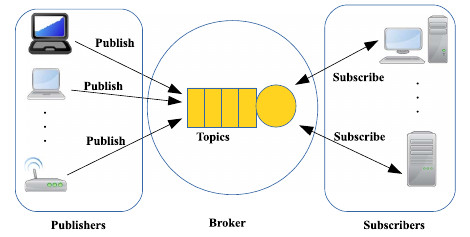
\includegraphics[width=0.8\textwidth]{imagens/mqtt.png}
  \label{fig:mqtt}  
  
  Fonte: \cite{Fuqaha2015}
\end{figure}

\paragraph*{DDS.} O DDS (Data Distribution Service) \cite{dds} é um protocolo de aplicação que também aplica o modelo publicador/observador, mas, ao contrário do MQTT, não envolve um elemento coordenador. Este protocolo prevê o envio de mensagens por \textit{multicast}, sendo adequado a redes com requisitos de tempo real no contexto de IoT, além de prover diversos parâmetros de qualidade de serviço.

A Tabela \ref{tab:comp_prot_aplic} resume as características principais dos protocolos de aplicação analisados. Observe que os protocolos apresentados se baseiam no TCP ou UDP, implicando em restrições quanto à sua utilização com protocolos de comunicação que não são baseados neles. 

\begin{table}[h]
	\centering
	\caption{Comparação dos Protocolos de Aplicação analisados}\smallskip
	\label{tab:comp_prot_aplic}
	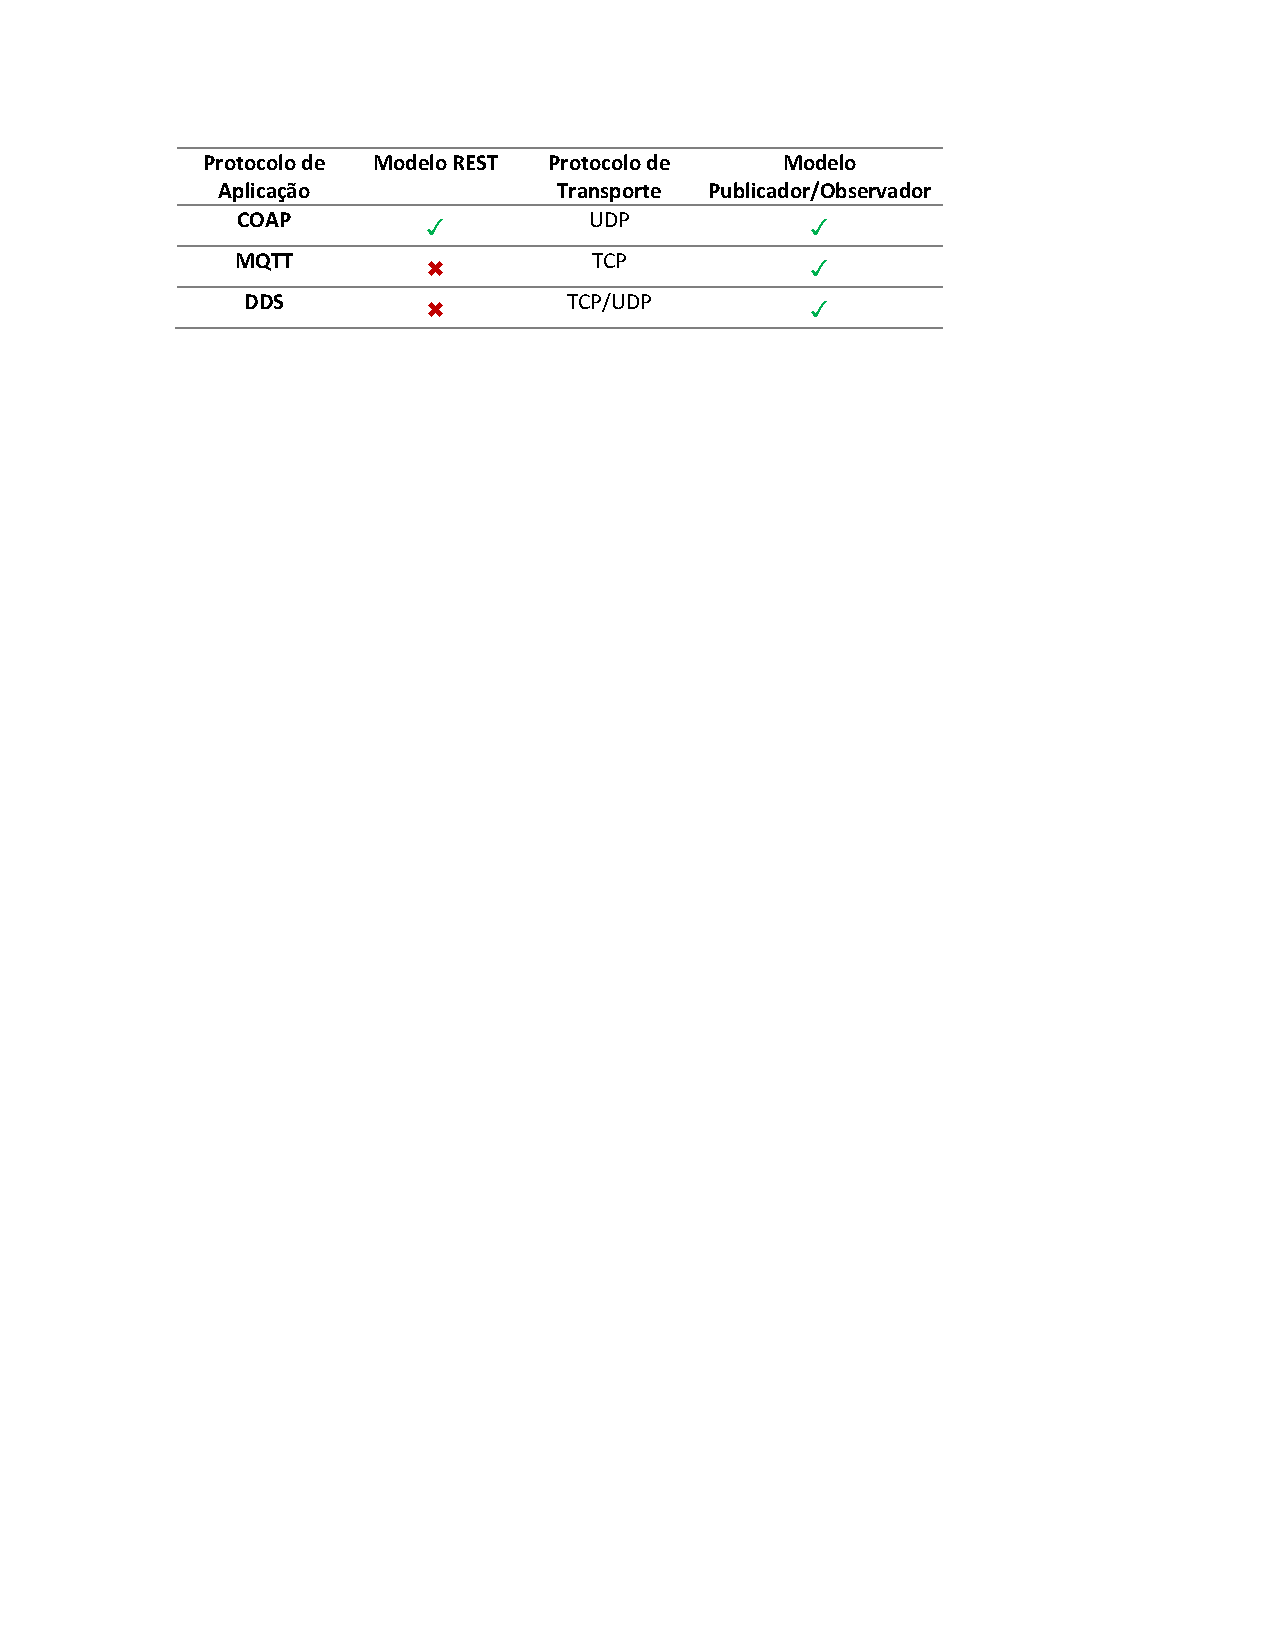
\includegraphics[width=\textwidth]{tabelas/comp_prot_aplic.pdf}
	
	Fonte: \cite{Fuqaha2015}
\end{table}

\subsection{\textit{Frameworks} existentes}
\paragraph*{IoTivity.} O IoTivity \cite{iotivity} é um projeto colaborativo da fundação Linux que tem por objetivo estabelecer um padrão para prover conectividade entre dispositivos no contexto de internet das coisas. Suas funcionalidades incluem possibilitar descoberta de dispositivos, transmissão de dados, gerenciamento de dispositivos e gerenciamento de dados, como ilustra a Figura \ref{fig:iotivity}. Seu funcionamento se baseia em uma arquitetura REST (baseado no CoAP), por meio da qual dados e mensagens de controle são trafegados. 

\begin{figure}[h]
	\centering
	\caption{Arquitetura do projeto IoTivity}
  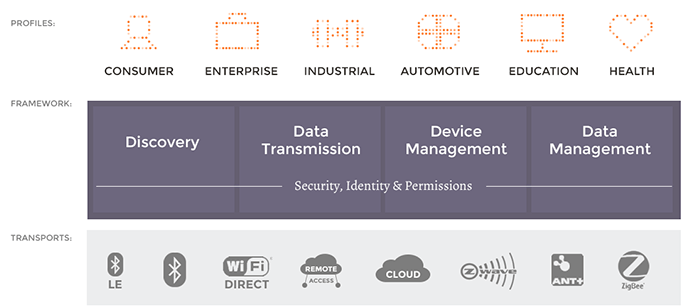
\includegraphics[width=0.8\textwidth]{imagens/iotivity.png}
  \label{fig:iotivity}  
  
  Fonte: \cite{iotivity}
\end{figure}

Uma característica proposta na arquitetura do IoTivity a ser adotada neste projeto é a criação de uma interface comum a vários protocolos de rede subjacentes, visto que provê flexibilidade à tecnologia de comunicação adotada pelos dispositivos. Entretanto, não se deseja adotar a abordagem REST utilizada no IoTivity, pois isso implica que todos os dispositivos necessitam escutar requisições continuamente. 

\paragraph*{ARM mbed.} O mbed \cite{mbed} é uma plataforma de desenvolvimento da ARM, que provê um ecossistema para desenvolvimento de aplicações em IoT. Um de seus produtos principais é o sistema operacional mbed OS, compatível somente com dispositivos baseados no microprocessador ARM Cortex-M. Este sistema provê um ambiente de execução baseado em eventos e suporta diversos protocolos de rede (Ethernet, Wi-Fi, 6loWPAN, Thread e Bluetooh LE), segurança e gerenciamento de dispositivos baseados em REST.

A plataforma mbed é relativamente complexa, provendo, além do sistema operacional citado, ferramentas de empacotamento de aplicações, de testes automatizados e de integração com serviços  em nuvem. Sua principal desvantagem é a restrição de processadores suportados, que apesar de ampla, restringe significativamente a flexibilidade dos dispositivos utilizados em uma rede. 

\paragraph*{RIOT.} O RIOT \cite{baccelli2013} é um sistema operacional que permite programar dispositivos utilizando  C ou C++, possibilitando utilizar ferramentas populares entre programadores como o compilador gcc e o depurador gdb. Ele provê suporte a diversas plataformas, além de prover implementações de diversas pilhas de rede (6LoWPAN, IPv6, UDP) e protocolos de aplicação tais como CoAP que podem ser incluídos nos programas caso necessários.

Uma desvantagem do RIOT é o fato de o seu uso estar restrito às plataformas suportadas, que apesar de estarem em expansão, não incluem, até o momento de escrita deste relatório, dispositivos de prototipação populares tais como o Arduino Uno e Raspberry Pi. Além disso, seu uso está restrito a processadores com um único núcleo, inviabilizando a utilização de dispositivos mais recentes. 
 
\section{Protocolos de rede existentes}\label{sec:commprot}
O projeto de uma rede de sensores e atuadores sem fio deve levar em conta diversas restrições dos dispositivos que a compõem, tais como o acesso limitado a uma fonte de energia, capacidade reduzida de processamento e meio de comunicação com interferências. Com estas restrições em mente, diversos protocolos de comunicação foram propostos para viabilizar a implementação de redes de sensores sem fio, descritos a seguir.

\subsection{ZigBee}
O ZigBee é um protocolo de comunicação proposto e padronizado pela \textit{ZigBee Alliance} em 2003, visando aplicação em redes de sensores sem fio \cite{zigbeealliance}. A especificação do protocolo abrange diversos aspectos, desde os de natureza física (e.g., estratégias de redução de intereferência) aos de aplicação (e.g., aplicação de criptografia sobre os dados transmitidos) \cite{stevanovic2007}. A Figura \ref{fig:zigbee} ilustra a abrangência do protocolo ZigBee, tendo como base um modelo em camadas de rede similar ao OSI.

\begin{figure}[h]
	\centering
	\caption{Abrangência da especificação do protocolo ZigBee, baseado em um modelo de camadas.}
  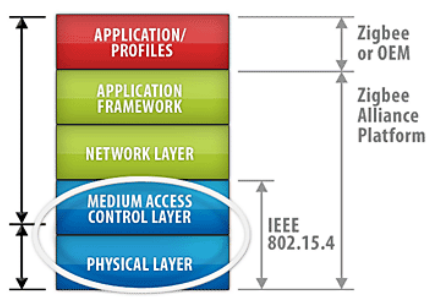
\includegraphics[width=0.8\textwidth]{imagens/zigbee.png}
  \label{fig:zigbee}
  
  Fonte: \cite{stevanovic2007}
\end{figure}

Como pode ser verificado no esquema, o ZigBee baseia-se na especificação IEEE 802.15.4 no que tange às camadas física e de controle de acesso ao meio (equivalente às camadas 1 e 2 do modelo OSI). O ZigBee define somente aspectos de alto nível que compõem as camadas de rede (camada 3) e de aplicação. Nos próximos parágrafos, será feita uma descrição do 802.15.4.

O protocolo IEEE 802.15.4 é um protocolo de camadas física e de enlace que busca prover comunicação com baixa complexidade para dispositivos com capacidades limitadas de transmissão de dados e de processamento \cite{ieee802_15}. A Tabela \ref{tab:802} resume as características deste protocolo.

\begin{table}[h]
	\centering
	\caption{Características do protocolo IEEE 802.15.4}\smallskip
	\label{tab:802}
	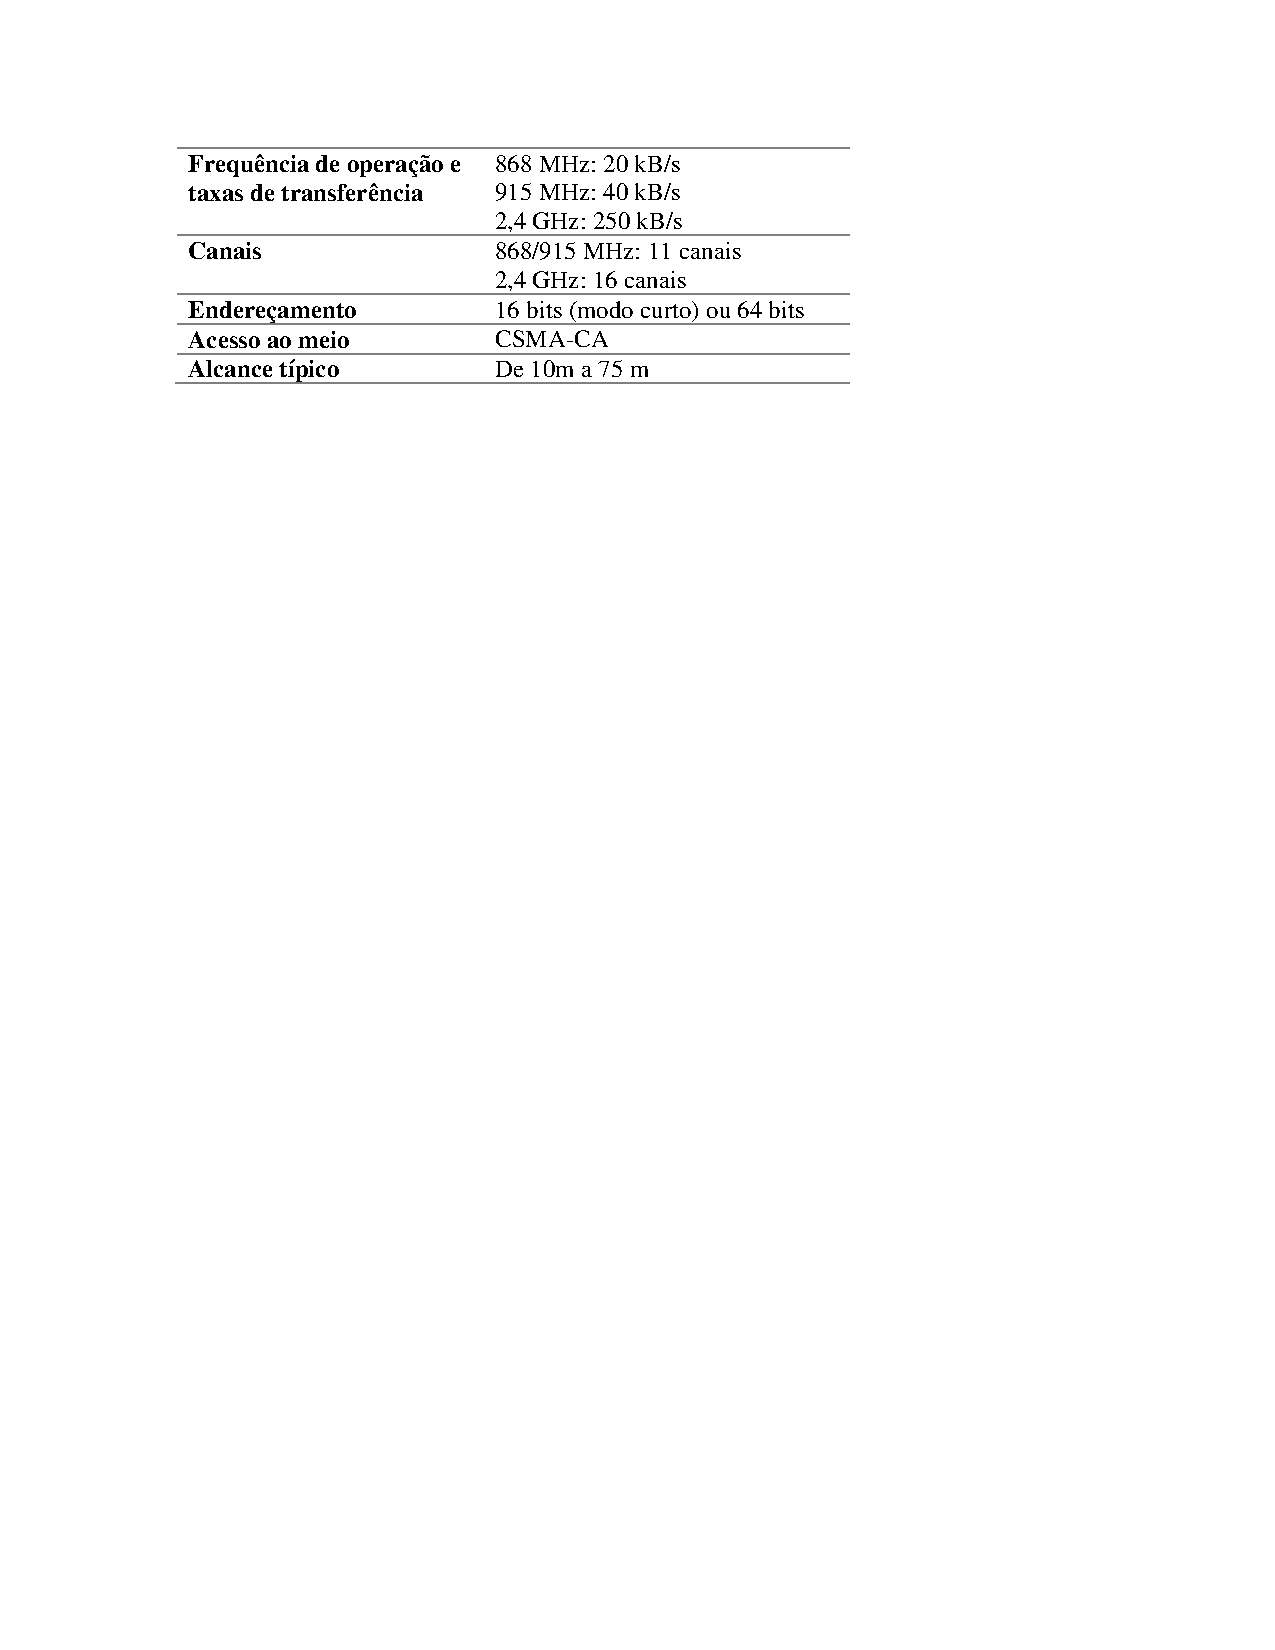
\includegraphics[width=0.8\textwidth]{tabelas/802_15_4.pdf}
	
	%\bigskip
	Fonte: \cite{stevanovic2007, schonwalder2010}
\end{table}
Como se pode notar, o protocolo opera em três faixas de frequência, sendo que a de 2,4 GHz provê maior número de canais e maior vazão de dados, além de estar licenciado para uso global, ao contrário das demais \cite{schonwalder2010}. Dentre as funções desempenhadas pelo 802.15.4, destacam-se o controle de acesso ao canal (baseado no CSMA-CA), a confirmação de entrega e checagem de erro em \textit{frames}.

O protocolo IEEE 802.15.4 ainda define dois tipos de dispositivos. Um dispositivo com funcionalidade completa (\textit{Full Function Device - FFD}) não possui restrições acentuadas de recursos, podendo se tornar um nó coordenador da rede de sensores. Ele pode efetuar diversas tarefas dentro da rede, tal como aceitar conexões e encaminhar pacotes. 

Um dispositivo com funcionalidade reduzida (\textit{Reduced Function Device - RFD}), por sua vez, consiste em um dispositivo periférico, tal como um sensor, possuindo restrições significativas de recursos. Estes dispositivos em geral atuam como ``folhas'' na topologia de rede, comunicando-se com um nó concentrador (um FFD) quando necessário.

Conforme mencionado, o ZigBee define recursos das camadas de rede e aplicação, como uma extensão ao protocolo 802.15.4 (ver Figura \ref{fig:zigbee}). Para tanto, são definidos três tipos de equipamentos dentro de uma rede ZigBee. Um dispositivo final consiste em um FFD ou RFD simples, que se comunica com um único nó. Um dispositivo roteador é um FFD capaz de reencaminhar mensagens  ao destinatário, caso necessário. Por fim, um dispositivo coordenador atua como coordenador da rede, possuindo também as funcionalidades de um roteador.

Pode-se derivar um recurso importante introduzido pela especificação do ZigBee: o roteamento \textit{multihop}, atuando como camada de rede. Isso significa que caso um dispositivo envie um pacote para outro que esteja fora do seu alcance, basta que haja roteadores conectando-os. Além disso, o ZigBee permite a formação de redes em malha (\textit{mesh}), provendo confiabilidade e tolerância a falhas.

Por fim, o ZigBee introduz recursos importantes em nível de aplicação. Exemplos incluem a possibilidade de fragmentação e remontagem de pacotes, manutenção de um registro de dispositivos pareados e funcionalidades relacionadas à segurança, como criptografia.

\subsection{6LoWPAN}
O 6LoWPAN é um protocolo definido pelo IETF que define a utilização de IPv6 sobre redes sem fio de baixo consumo, de alcance pessoal (acrônimo do inglês \textit{IPv6 over Low-power Wireless Personal Area Network}) \cite{rfc4944}. O objetivo principal deste protocolo é integrar o protocolo IP em redes de baixo consumo, trazendo diversos benefícios, tais como \cite{rfc4919, schonwalder2010}
\begin{itemize}
	\item A possibilidade de se reutilizar a infraestrutura IP existente;
	\item A possibilidade de adotar tecnologias que trabalham sobre o protocolo IP, em geral amplamente conhecidos e aceitos por profissionais;
	\item A facilidade de interoperabilidade com redes IP existentes, e
	\item A adequação do esquema de endereçamento do IPv6, suprindo a necessidade de um grande número de endereços exigido em uma aplicação de IoT.
\end{itemize}

De modo semelhante ao ZigBee, o 6LoWPAN baseia-se no protocolo IEEE 802.15.4 no que tange às camadas física e de enlace, de modo a se adequar a redes de baixo consumo. No entanto,o 6LoWPAN define uma camada de interface entre as camadas do 802.15.4 e IP, como pode ser visto na Figura \ref{fig:6lowpan}.

\begin{figure}[h]
	\centering
	\caption{A especificação do protocolo 6LoWPAN e sua relação com os protocolos 802.15.4 e IP. O modelo OSI é mostrado ao lado como referência.}
  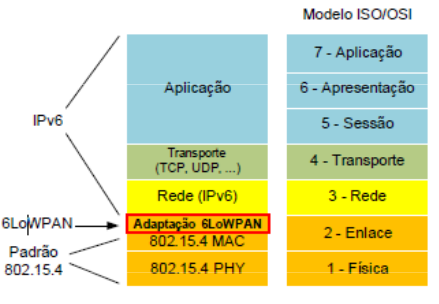
\includegraphics[width=0.8\textwidth]{imagens/6lowpan.png}
  \label{fig:6lowpan}
  
  Fonte: \cite{moreiras2009}
\end{figure}

A necessidade de uma camada de interface entre o IPv6 e as camadas inferiores padronizadas pelo 802.15.4 se dá por incompatibilidades existentes entre tais protocolos \cite{rfc4919}. Um exemplo diz respeito ao tamanho dos pacotes previstos por cada protocolo: o 802.15.4 prevê pacotes pequenos, com tamanhos de no máximo 81 bytes, ao passo que o IPv6 exige suporte a um MTU mínimo de 1280 bytes. Logo, um papel da interface definida pelo 6LoWPAN é o de efetuar fragmentação e montagem dos pacotes, a fim de compatibilizar os protocolos.
Outras funções do protocolo incluem:
\begin{itemize}
	\item Compressão de cabeçalho: como mencionado, o 802.15.11 suporta cabeçalhos de no máximo 81 bytes. Sendo que um cabeçalho IPv6 ocupa no mínimo 40 bytes (sem os cabeçalhos opcionais), restam somente 41 bytes para serem usados pelos protocolos de camadas superiores. Fica evidente, então, a necessidade de se aplicar técnicas de compressão de cabeçalho, função esta desempenhada pelo 6LoWPAN;
	\item Roteamento \textit{multi-hop} em redes \textit{mesh}: de modo semelhante ao ZigBee, o 6LoWPAN permite a configuração de redes \textit{mesh} com capacidade de  autorreparação, provendo robustez.
\end{itemize}

\subsection{Bluetooth}
Bluetooth é uma tecnologia de comunicação sem fio a curta distância. Opera em banda não licenciada ISM (Industrial, Científica e Médica, na sigla em inglês) entre 2,4Ghz e 2,485GHz.
Por não utilizar banda licenciada, o Bluetooth utiliza saltos adaptativos em frequência (\textit{Adaptative Frequency Hopping} - AFH) para diminuir a interferência com outros dispositivos operantes na mesma faixa de 2,4GHz. O aparelho toma conhecimento de demais dispositivos na mesma frequência e as evita, saltando entre 79 frequências a intervalos de 1MHz \cite{redesbluetooth}. 

A operação Bluetooth ocorre em redes Ad-Hoc de curto alcance conhecidas como Piconet. Tais redes podem ser constituídas por 1 membro mestre, 7 escravos ativos e 248 escravos estacionados (endereçamento de 8 bits). Cada dispositivo pode pertencer a várias Piconets. 
Seu raio de operação depende do dispositivo utilizado, que pode ser classificado em três categorias:
\begin{itemize}
        \item Classe 3: alcance de 1 metro e potência máxima de 1mW.
        \item Classe 2: alcance de 10 metros e potência máxima de 2,5mW.
        \item Classe 1: alcance de 100 metros, potência máxima de 100mW.
\end{itemize}

A camada mais baixa da arquitetura Bluetooth é a camada Física, na qual são definidas as especificações do dispositivo para operar. Dois dispositivos compartilham o mesmo meio físico e para se comunicarem devem estar sintonizados na mesma frequência (processo de parear). Para identificar os membros da Piconet, um código de acesso é sempre enviado no cabeçalho de cada pacote, aumentando a carga e inviabilizando para dispositivos de menor capacidade, como no caso deste projeto. 

Uma mesma unidade pode participar como escrava em várias Piconets mas atuar como mestre em apenas uma. Para participar de mais de uma Piconet o dispositivo atua com multiplexação no tempo (\textit{Time Division Multiplexing} - TDM). O conjunto de várias Piconets independentes e não sincronizadas é chamado de Scatternet, conforme esquematizado na Figura \ref{fig:redesbluetooth}.

\begin{figure}[h]
	\centering
	\caption{Diagrama para rede Piconet e conjunto gerando Scatternet.}
  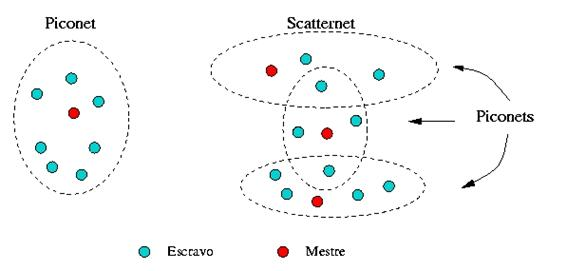
\includegraphics[width=0.8\textwidth]{imagens/redesbluetooth.jpg}
  \label{fig:redesbluetooth}
  
  Fonte: \cite{redesbluetooth}
\end{figure}

No acesso ao meio físico utiliza-se o método CDMA (\textit{Code Division Multiple Access}). Para o projeto da casa conectada, utilizaria-se o padrão de Enlace ACL (\textit{Asynchronous Conection-Less}), do tipo ponto-multiponto (um mestre e vários escravos). Este padrão é adequado para transmissão de dados, de modo que pacotes perdidos ou com erros são retransmitidos. 

Em qualquer rede sem fio, a vulnerabilidade das informações é evidente. Como o meio que propaga o sinal é o próprio ar, um dispositivo pode captar um sinal sendo enviado se este não for devidamente protegido. No caso da tecnologia Bluetooth, onde as conexões são feitas de forma automática, é especialmente importante definir formas de proteger os usuários para que não recebam dados de dispositivos que não desejam.

Para garantir a integridade das informações, aplicam-se modos de criptografia e autenticação. Isto é especialmente importante no projeto da casa conectada, no qual usuários externos e diferentes do dono do sistema não podem ter acesso aos dados trafegados. 

Para iniciar uma conexão, um pedido de permissão deve ser enviado. Os dispositivos Bluetooth usam uma chave de acesso chamada número de identificação pessoal (PIN) para autenticação. Se a chave de acesso digitada pelo usuário que deseja conectar corresponder à chave de acesso ao dispositivo detectado, a autenticação é realizada com êxito. Caso contrário ela falhará. 

\subsection{Z-Wave}
Z-Wave é um protocolo de comunicação sem fio que tem como foco baixo consumo, baixa taxa de dados e confiabilidade. Foi criado pela empresa dinamarquesa Zen-Sys, que foi adquirida pela Sigma Designs e desde sua concepção é voltada para automação residencial \cite{wikizwave,zwavelayers}.

As duas camadas mais baixas (Física e Enlace) da pilha de protocolos são definidas pelo ITU-T G.9959, ou seja, trata-se de um padrão formalmente definido por um órgão internacional de padrões. Porém, sua camada de rede é definida pela Sigma Designs e as camadas acima são definidas pelo desenvolvedor da aplicação, como pode ser observado na Figura \ref{fig:zwavelayers}.


\begin{figure}[h]
	\centering
	\caption{Pilha de protocolos do Z-Wave}
  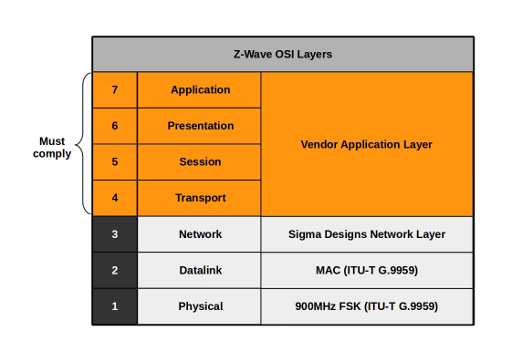
\includegraphics[width=0.8\textwidth]{imagens/zwavelayers.jpg}
  \label{fig:zwavelayers}
  
    Fonte: \cite{zwavelayers}
\end{figure}

O Z-Wave trabalha em frequências abaixo de 1GHz, por volta de 900MHz, fazendo com que ela não interfira com Wi-Fi, Bluetooth e diversas outras tecnologias que trabalham na já bastante utilizada frequência de 2,4GHz. Além disso, suas taxas de transmissão são de 9600 bit/s, 40 kbit/s ou 100 kbit/s e seu alcance é de 100m em áreas abertas.

Uma rede Z-Wave define dois tipos de dispositivos: controladores e escravos. Os controladores iniciam comandos de controle para os escravos e os enviam. Já os nós escravos apenas respondem a comandos e os executam. Porém, estes nós também podem funcionar como repetidores, aumentando o alcance de sua rede Z-Wave.

Cada rede Z-Wave pode conter até 232 dispositivos e é identificada por um ID da rede (Network ID ou Home ID), que possui 32 bits. Nós conectados em redes distintas não podem se comunicar diretamente entre si, e em uma rede cada nó tem um ID único (Node ID) de 8 bits.

As redes Z-Wave utilizam uma topologia de malha (\textit{mesh}) e é necessário existir um controlador primário e opcionalmente controladores secundários. Os nós são adicionados através do pareamento em que o controlador mede a força do sinal entre os equipamentos e assume que esta irá se manter constante, fazendo com que os escravos não possam se mover espacialmente sem terem que realizar o pareamento novamente.

%\section{Análise dos protocolos de comunicação}
%Uma vez descritos os protocolos de comunicação, é possível analisar as vantagens e desvantagens de cada um deles, tendo em vista o escopo do presente trabalho. A Tabela \ref{tab:analiseprotcom} lista de forma sucinta as características levantadas de cada protocolo.
%
%\begin{table}[h]
%	\centering
%	\caption{Análise dos protocolos de comunicação}\smallskip
%	\label{tab:analiseprotcom}
%	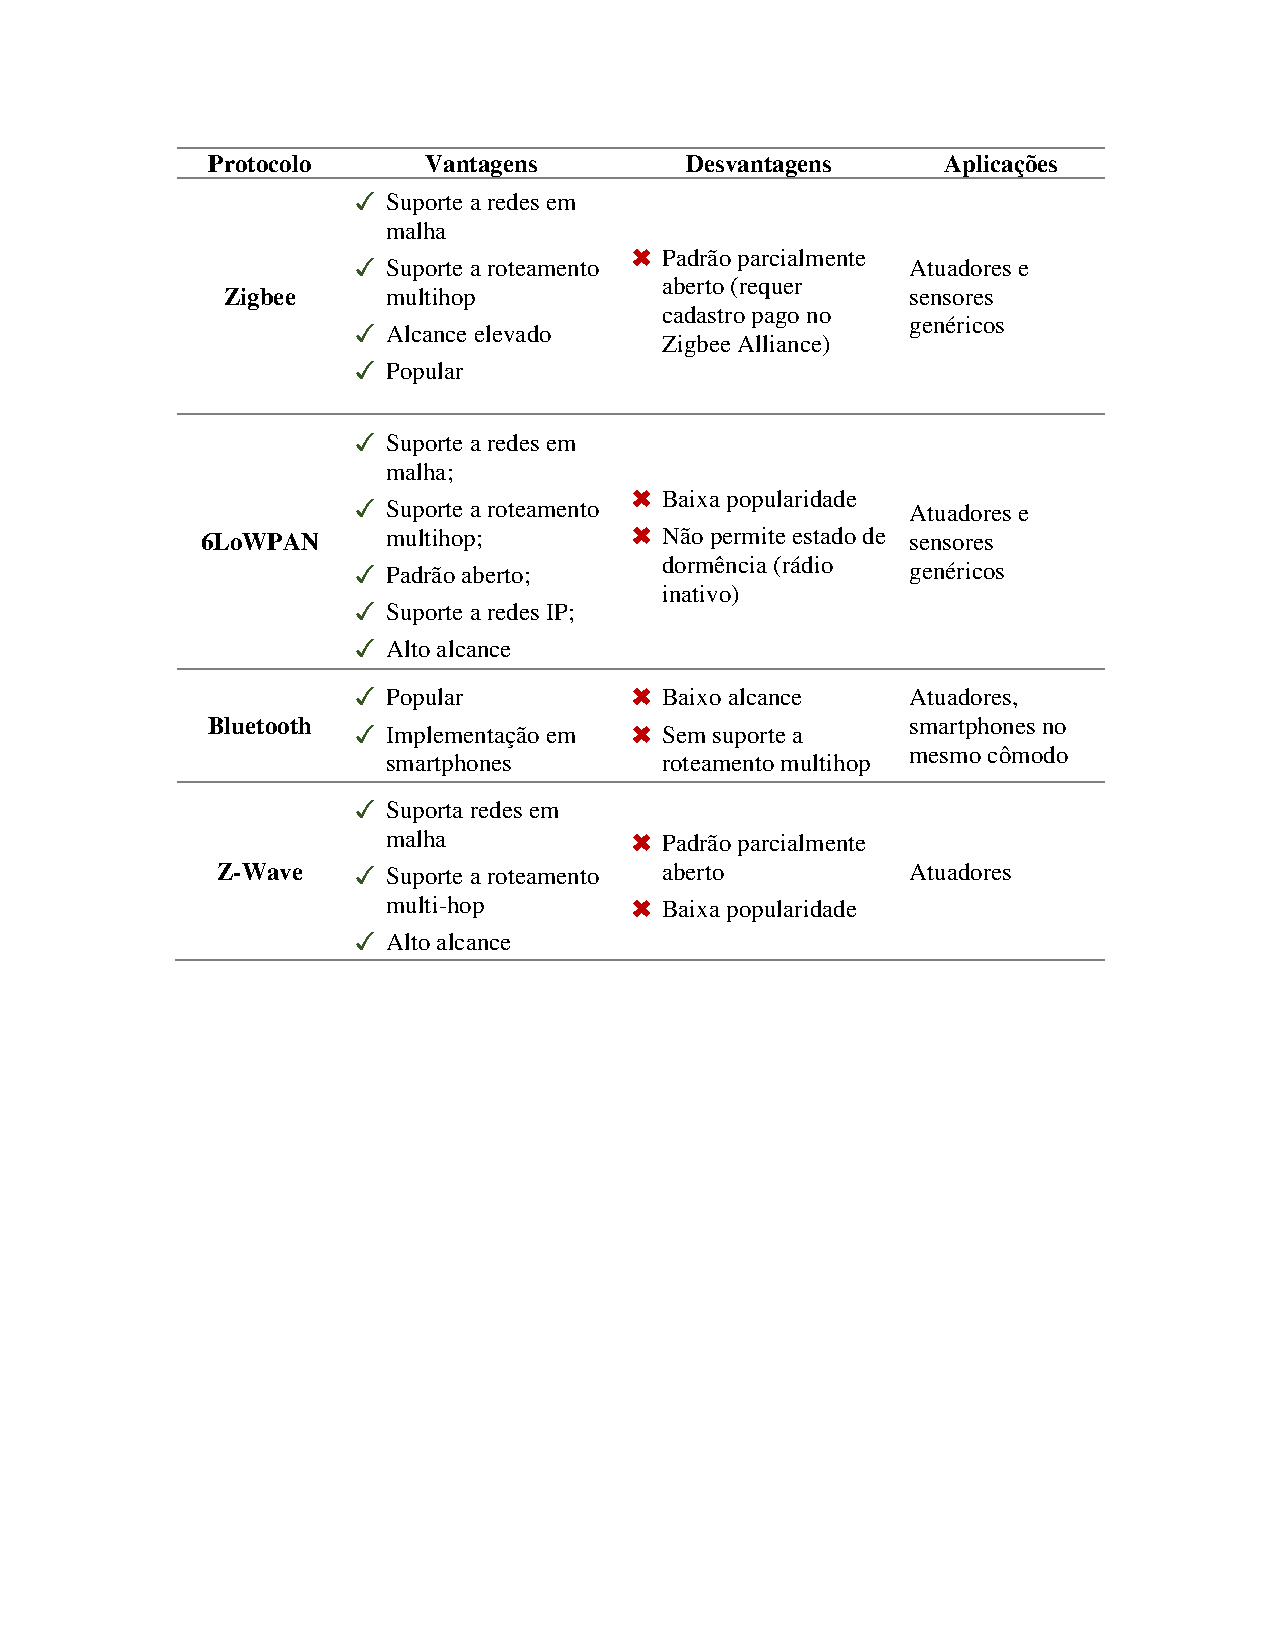
\includegraphics[width=\textwidth]{tabelas/comp_prot_rede.pdf}
%\end{table}
%
%Conforme mencionado, os protocolos ZigBee e 6LoWPAN são baseados no padrão IEEE 802.15.4, apresentando, pois, características físicas e de acesso ao meio similares, tais como frequência de operação e alcance. Ambos ainda preveem suporte a redes em malha com roteamento \textit{multihop}, permitindo aplicações em ambientes em que a localização dos dispositivos seja esparsa, sendo necessário roteadores intermediários para comunicação.
%
%No entanto, tais protocolos diferem entre si em alguns aspectos. Em primeiro lugar, o ZigBee foi padronizado em 2003, visto como o protocolo mais popular utilizado em redes de sensores sem fio \cite{toscano2012}. O 6LoWPAN, por sua vez, é um padrão mais novo, tendo sido proposto pelo IETF em 2007. Além disso, a especificação do 6LoWPAN é totalmente aberta, além de adotar camadas de nível superior (rede e transporte) conhecidas e amplamente adotadas em redes existentes (IP e TCP/UDP), ao passo que o ZigBee define camadas de rede e aplicação próprias, em uma especificação de acesso restrito. Por fim, o Zigbee prevê a possibilidade de os nós entrarem em um estado de dormência (rádio inativo), ao passo que o 6LoWPAN não permite este modo. Isto se deve ao fato de ele estar baseado no protocolo IP, que prevê que os nós sempre estejam ativos \cite{toscano2012}.
%
%Em relação ao Bluetooth, pode-se considerá-lo um protocolo amplamente difundido, sendo integrado inclusive em maior parte dos dispositivos móveis atuais. No entanto, ele possui a desvantagem de possuir alcance limitado e de não suportar redes complexas, limitando a abrangência da rede. Soma-se a isso o fato de não ser possível iniciar a comunicação de um dispositivo escravo a um mestre (coordenador), tornando inconveniente a utilização de sensores como escravos, haja vista a necessidade de mantê-los ativos à espera de uma mensagem do dispositivo mestre para envio das leituras.
%
%Por fim, nota-se que o Z-Wave possui vantagens em comum às do ZigBee e do 6LoWPAN. Em contrapartida, sua especificação é parcialmente aberta, além de possuir baixa adoção. De modo similar ao Bluetooth, este dispositivos atuando como escravos não podem iniciar uma comunicação, devendo somente responder às mensagens de um mestre.

%Ponderando as características expostas, o grupo optou por adotar o protocolo ZigBee para implementar um protótipo de rede a ser utilizado como base para projetar o protocolo de nível de aplicação. Cabe ressaltar que o protocolo de aplicação deve ser genérico a ponto de funcionar corretamente independente da escolha dos protocolos de comunicação subjacentes.

\section{Definição do Protocolo de Aplicação \textit{Rainfall}}
\subsection{Requisitos} \label{subsec:requisitos}
Uma vez analisados os protocolos de aplicação e frameworks existentes (seção \ref{sec:relwork}), bem como os protocolos de rede (seção \ref{sec:commprot}), e tendo em vista os requisitos levantados para a rede de sensores (seções \ref{sec:reqfunc} e \ref{sec:reqnfunc}), pode-se passar para a especificação do protocolo de aplicação proposto, batizado de \textit{Rainfall}.

\begin{enumerate}[\quad R1.]
	\item O protocolo a ser desenvolvido deve funcionar com diversos protocolos de rede. Conforme a análise realizada, existem diversos protocolos de redes voltados a redes de sensores sem fio existentes, e convém que o protocolo de aplicação desenvolvido não seja restrito a nenhum deles de forma específica. Uma abordagem similar à do IoTivity pode ser interessante, criando-se uma interface comum a vários protocolos de rede subjacentes;
	\item Os dispositivos devem poder declarar sua funcionalidade, incluindo informações sobre sua classificação como sensor ou atuador, e sua categoria (tipo de sensor ou atuador);
	\item Os dispositivos devem poder enviar dados de leitura (no caso de sensores) e receber comandos de atuação (no caso de atuadores);
	\item O protocolo deve enviar mensagens de forma concisa, levando em consideração as limitações dos dispositivos envolvidos.
\end{enumerate}

\subsection{Sintaxe e Semântica} \label{subsec:sintaxe}
Levando-se em conta a natureza das mensagens a serem transmitidas, convém adotar uma estrutura de dados no formato chave-valor. Neste relatório, a representação dos dados seguindo este formato será feito de forma similar ao formato JSON:
\begin{center}
	\texttt{\{chave\_1:valor\_1, ..., chave\_n:valor\_n\}}
\end{center}
onde \texttt{chave\_1}, \texttt{chave\_n} são as chaves e \texttt{valor\_1}, \texttt{valor\_n} são os valores associados.

Os requisitos definidos na seção \ref{subsec:requisitos} permitem definir as chaves e valores associados a serem utilizados no protocolo, conforme mostra a Tabela \ref{tab:chavevalorprot}.

\begin{table}[h]
	\centering
	\caption{Chaves e valores associados utilizados no protocolo de aplicação.}\smallskip
	\label{tab:chavevalorprot}
	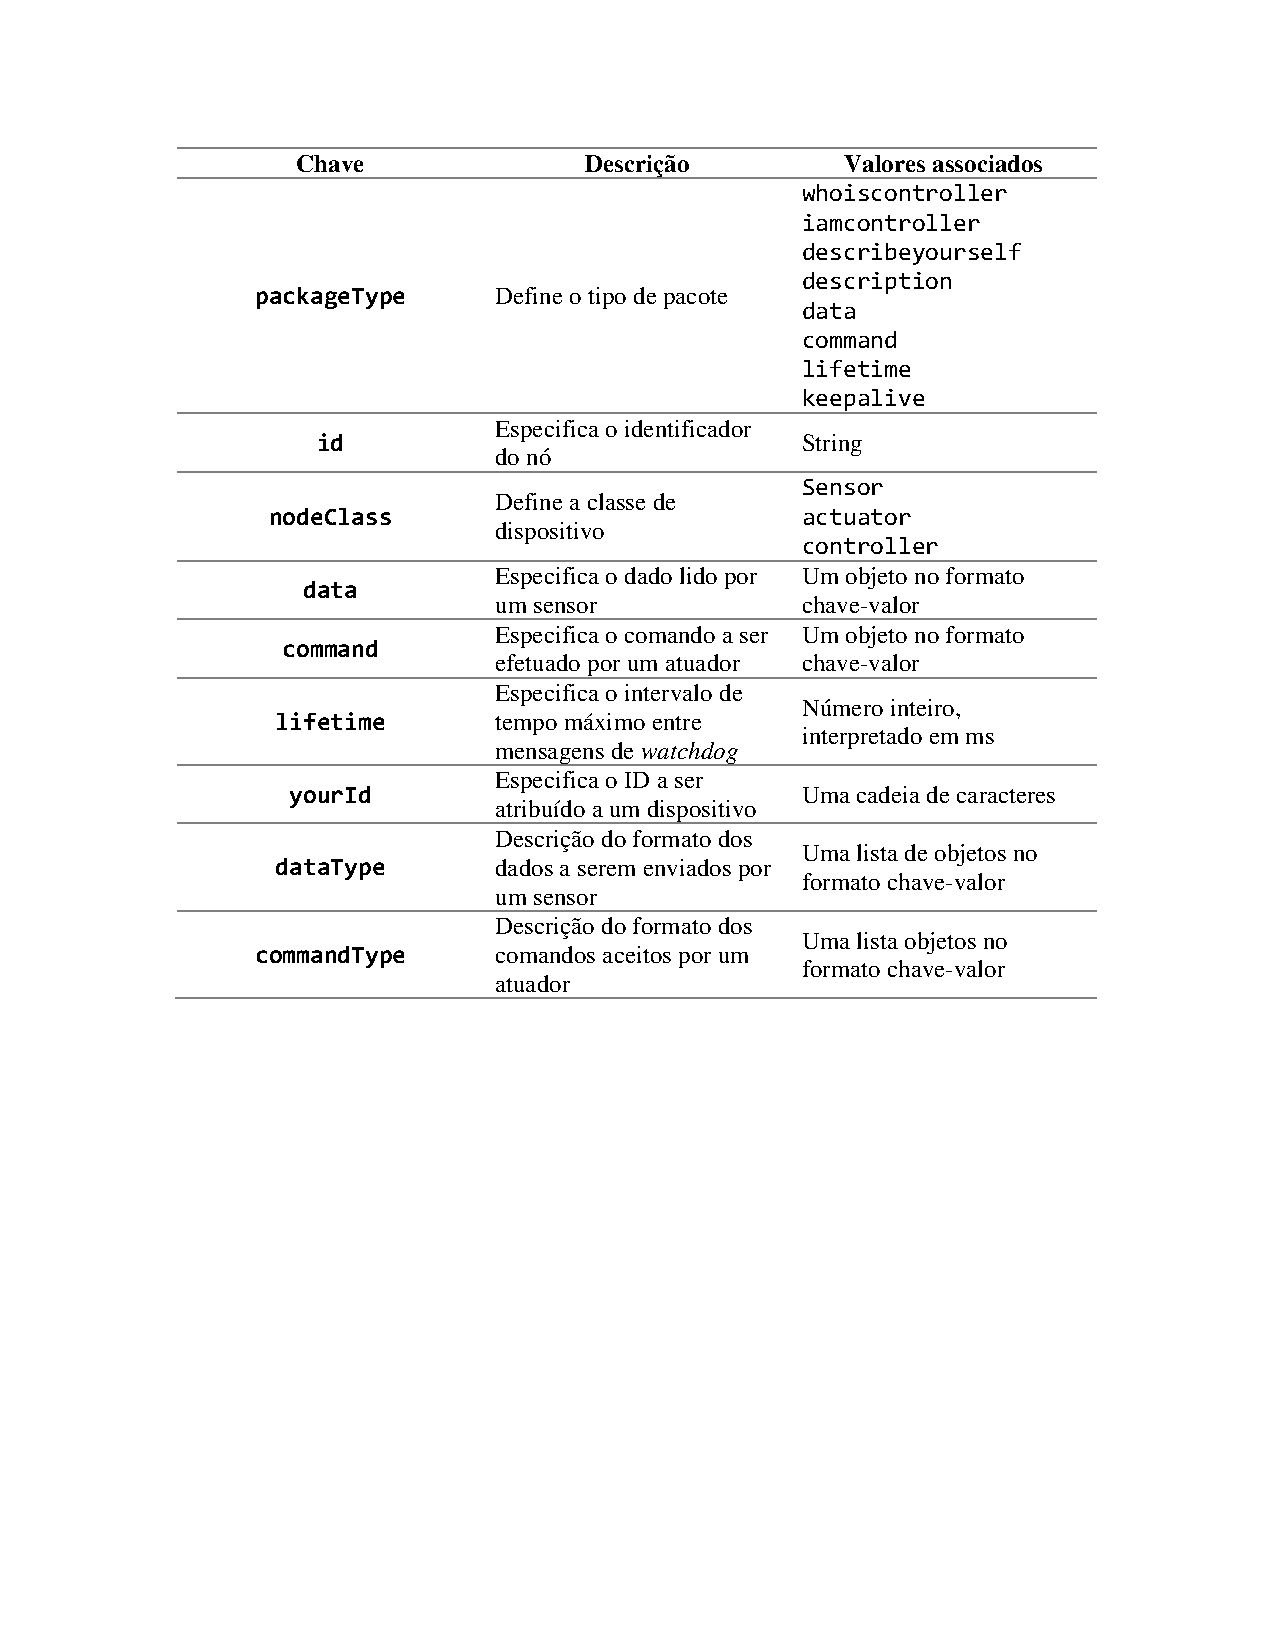
\includegraphics[width=0.9\textwidth]{tabelas/chave_valor_prot.pdf}
\end{table}

A chave \texttt{packageType} descreve o tipo do pacote, definindo os demais campos que devem estar presentes nele e como devem ser interpretados. Os possíveis valores dessa chave são:

\paragraph*{\texttt{whoiscontroller}.} Esta mensagem é enviada por um dispositivo sensor ou atuador  por broadcast para descobrir o endereço do controlador. 

\paragraph*{\texttt{iamcontroller}.} Mensagem enviada em resposta ao pedido de descoberta de controlador. Espera-se que este pacote conte com o seguinte campo:
\begin{itemize}
	\item \texttt{yourId}: esta mensagem é emitida pelo controlador, definindo o identificador a ser utilizado pelos dispositivos da rede nas comunicações subsequentes.
\end{itemize}

\paragraph*{\texttt{describeyourself}.} Mensagem enviada pelo controlador solicitando ao dispositivo-alvo uma descrição de suas funcionalidades.

\paragraph*{\texttt{description}.} Consiste na descrição das funcionalidades do dispositivo, enviada em resposta ao pedido \texttt{describeyourself}. Espera-se que um pacote deste tipo conte com os seguintes campos:
\begin{itemize}
	\item \texttt{nodeClass}: define a classe de um dispositivo, que pode ser sensor, atuador ou controlador. Um sensor é definido como um dispositivo que envia dados de leitura. Um controlador é um dispositivo que recebe comandos e efetua ações baseadas neles. Um controlador é um dispositivo que coordena sensores e atuadores, recebendo dados de leitura e enviando comandos de atuação;
	\item \texttt{dataType}: especifica as classes de dados que são emitidos pelo sensor. Consiste em um objeto com chaves e valores definidos conforme mostra a Tabela \ref{tab:datatype}. O campo \texttt{category} define a categoria de dados coletados pelo sensor, além de especificar os tipos que podem ser alocados no campo \texttt{type}. A Tabela \ref{tab:classesdados} define os valores possíveis de serem utilizados como categoria, além de listar os tipos de dados permitidos para cada categoria;
	\item \texttt{commandType}: especifica as classes de comandos aceitos pelo atuador. Consiste em um objeto com chaves e valores definidos conforme mostra a Tabela \ref{tab:commandtype}. O campo \texttt{category} define a categoria de comandos aceitos pelo atuador, além de especificar os tipos que podem ser alocados no campo \texttt{type}. A Tabela \ref{tab:classescomandos} define os valores possíveis de serem utilizados como categoria, além de listar os tipos de dados permitidos para cada categoria.
\end{itemize}

\begin{table}[hp]
	\centering
	\caption{Chaves e valores associados utilizados na declaração de tipos de dados lidos por um sensor.}\smallskip
	\label{tab:datatype}
	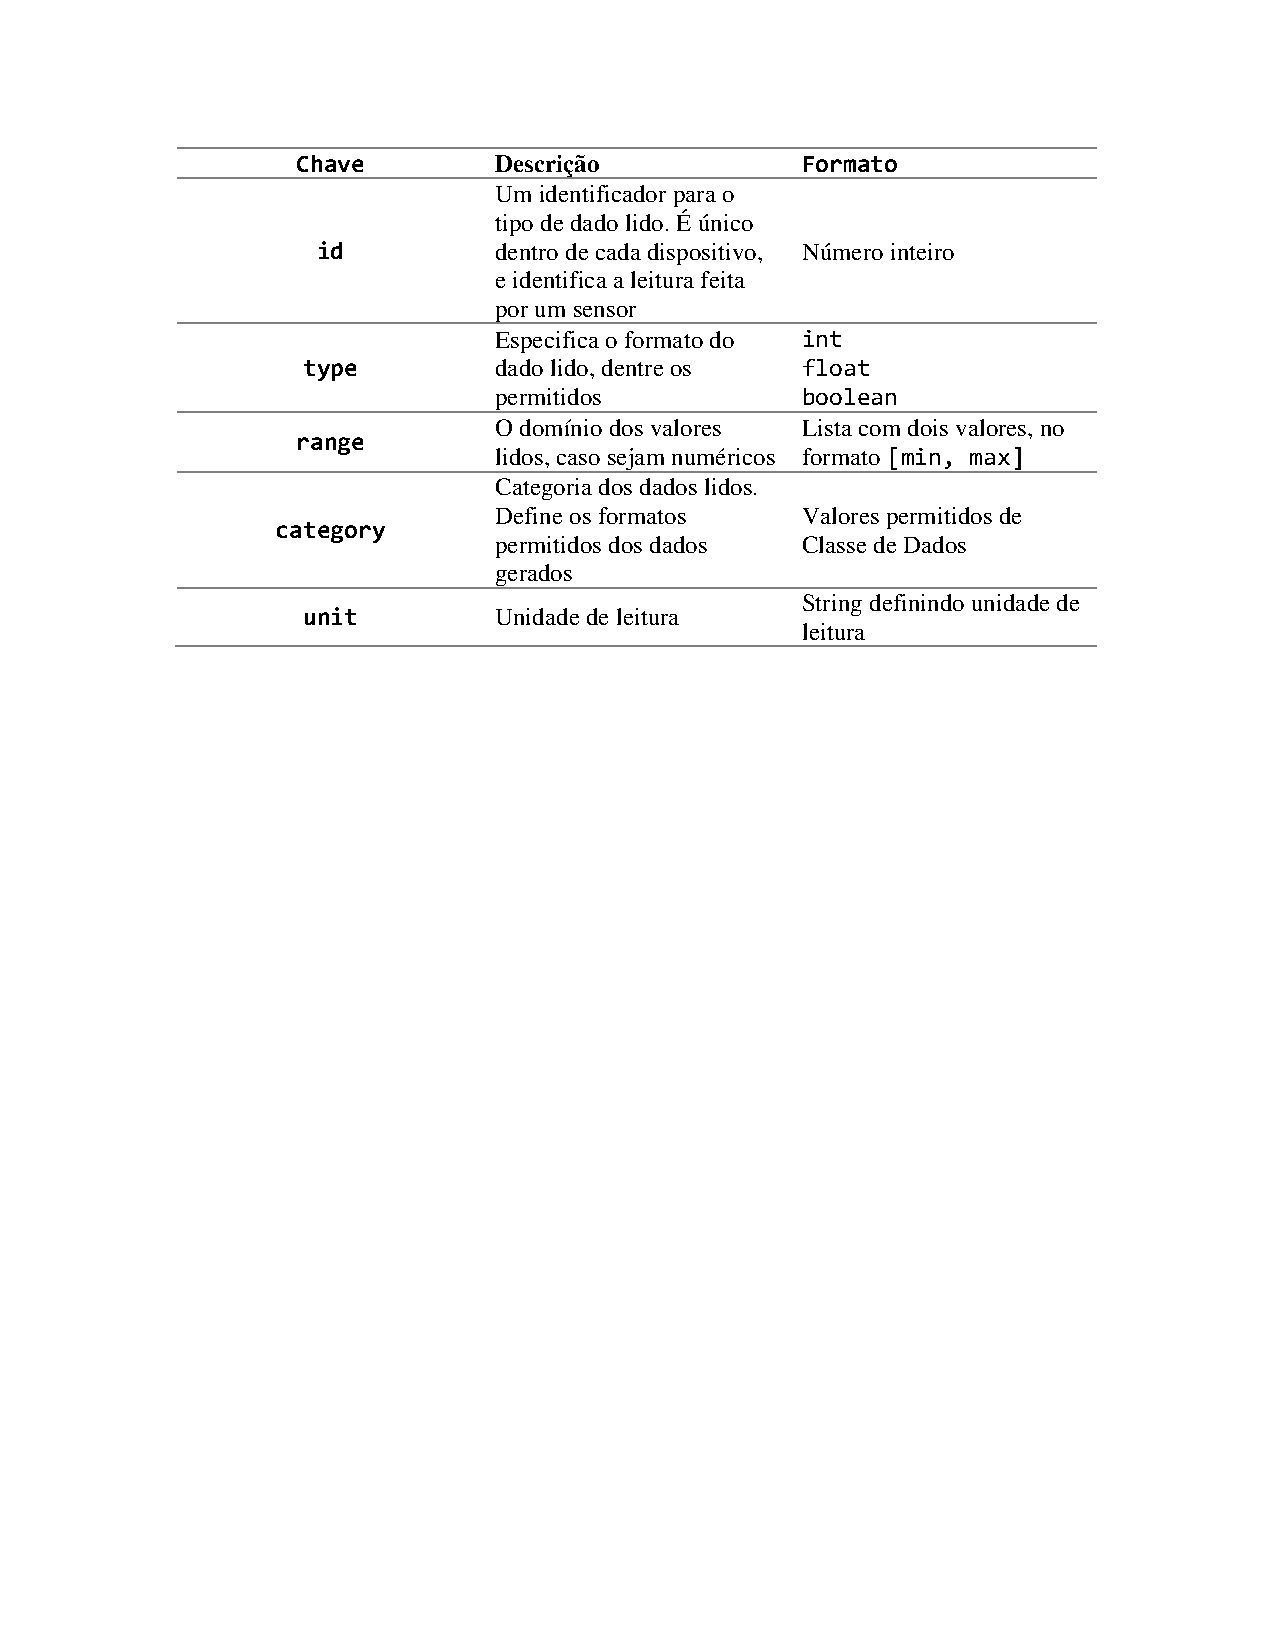
\includegraphics[width=0.9\textwidth]{tabelas/datatype.pdf}
	
	\medskip
	
	\caption{Categorias de dados e os respectivos tipos de valores permitidos.}\smallskip
	\label{tab:classesdados}
	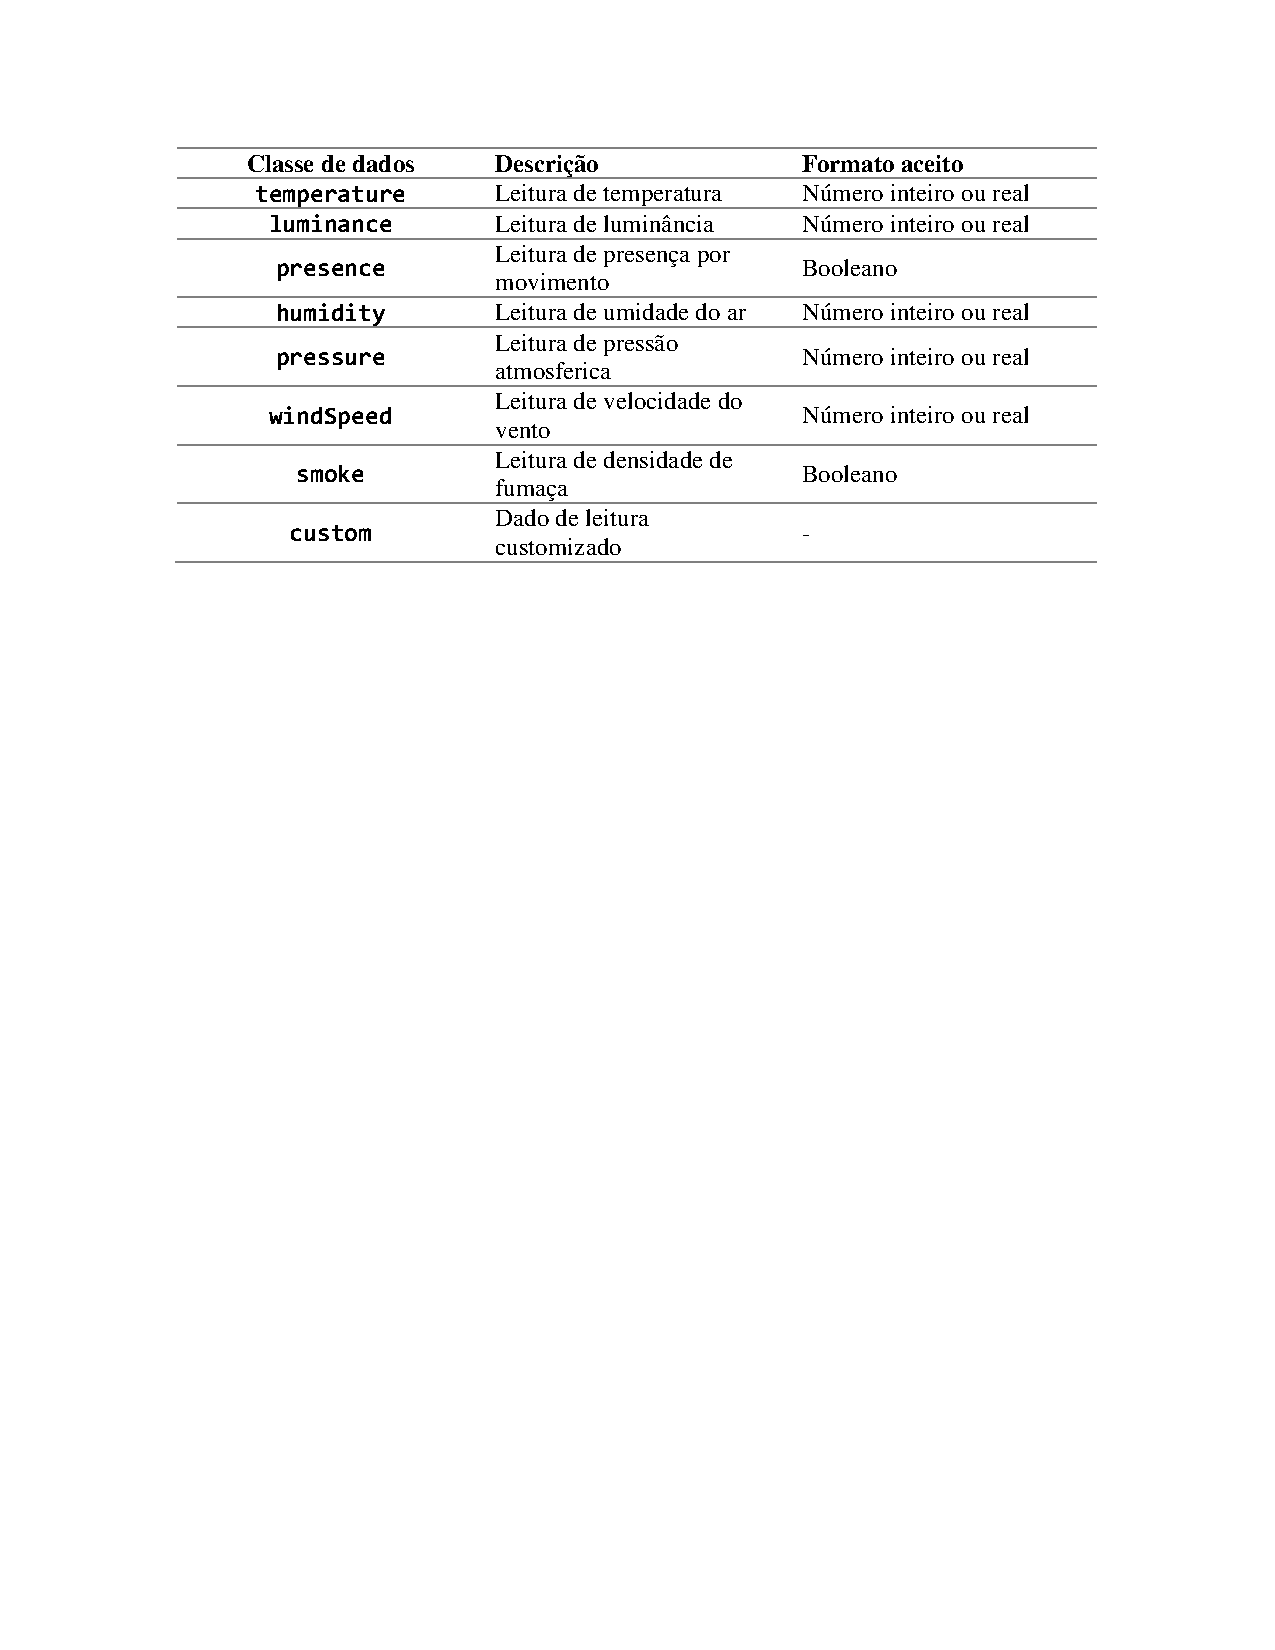
\includegraphics[width=0.9\textwidth]{tabelas/classes_dados.pdf}
\end{table}

\begin{table}[hp]
	\centering
	\caption{Chaves e valores associados utilizados na declaração de tipos de comandos aceitos por um atuador.}\smallskip
	\label{tab:commandtype}
	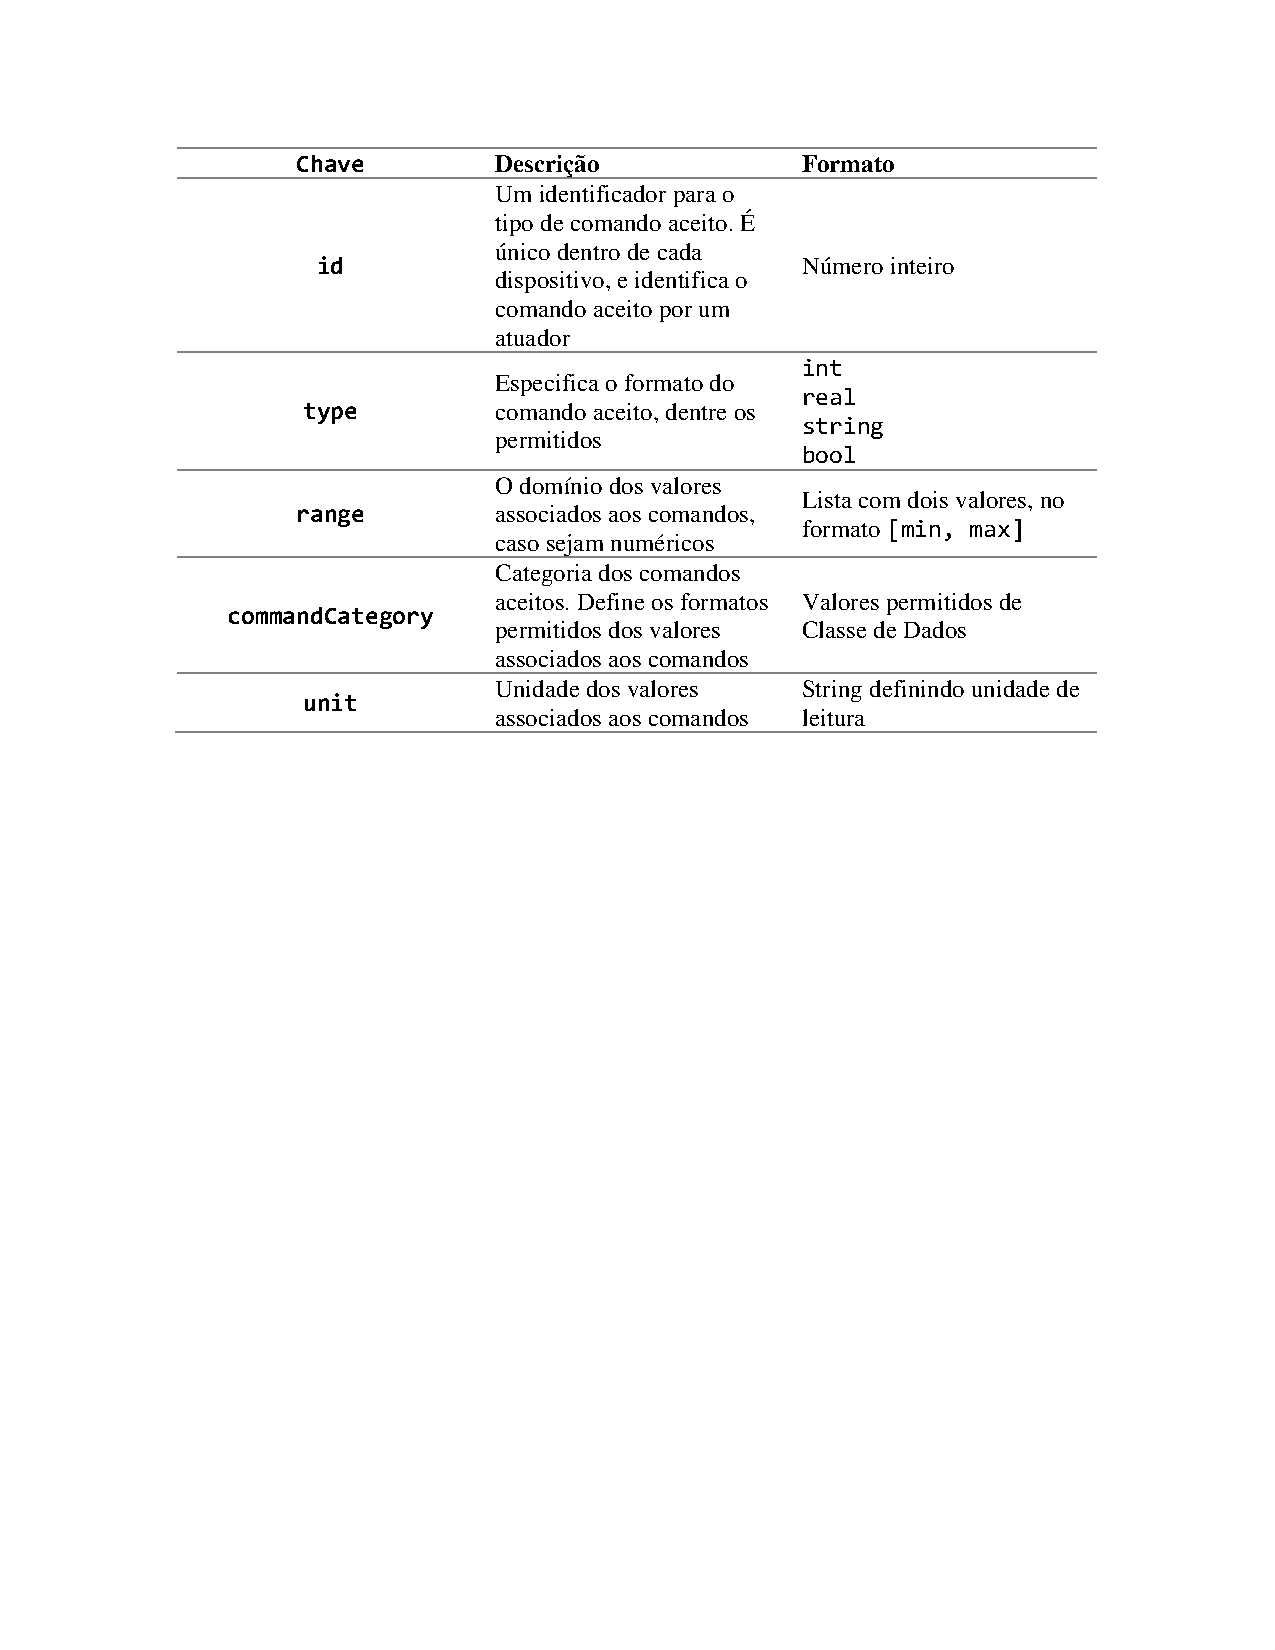
\includegraphics[width=0.9\textwidth]{tabelas/commandtype.pdf}
	
	\medskip
	
	\caption{Categorias de comandos e os respectivos tipos de valores permitidos.}\smallskip
	\label{tab:classescomandos}
	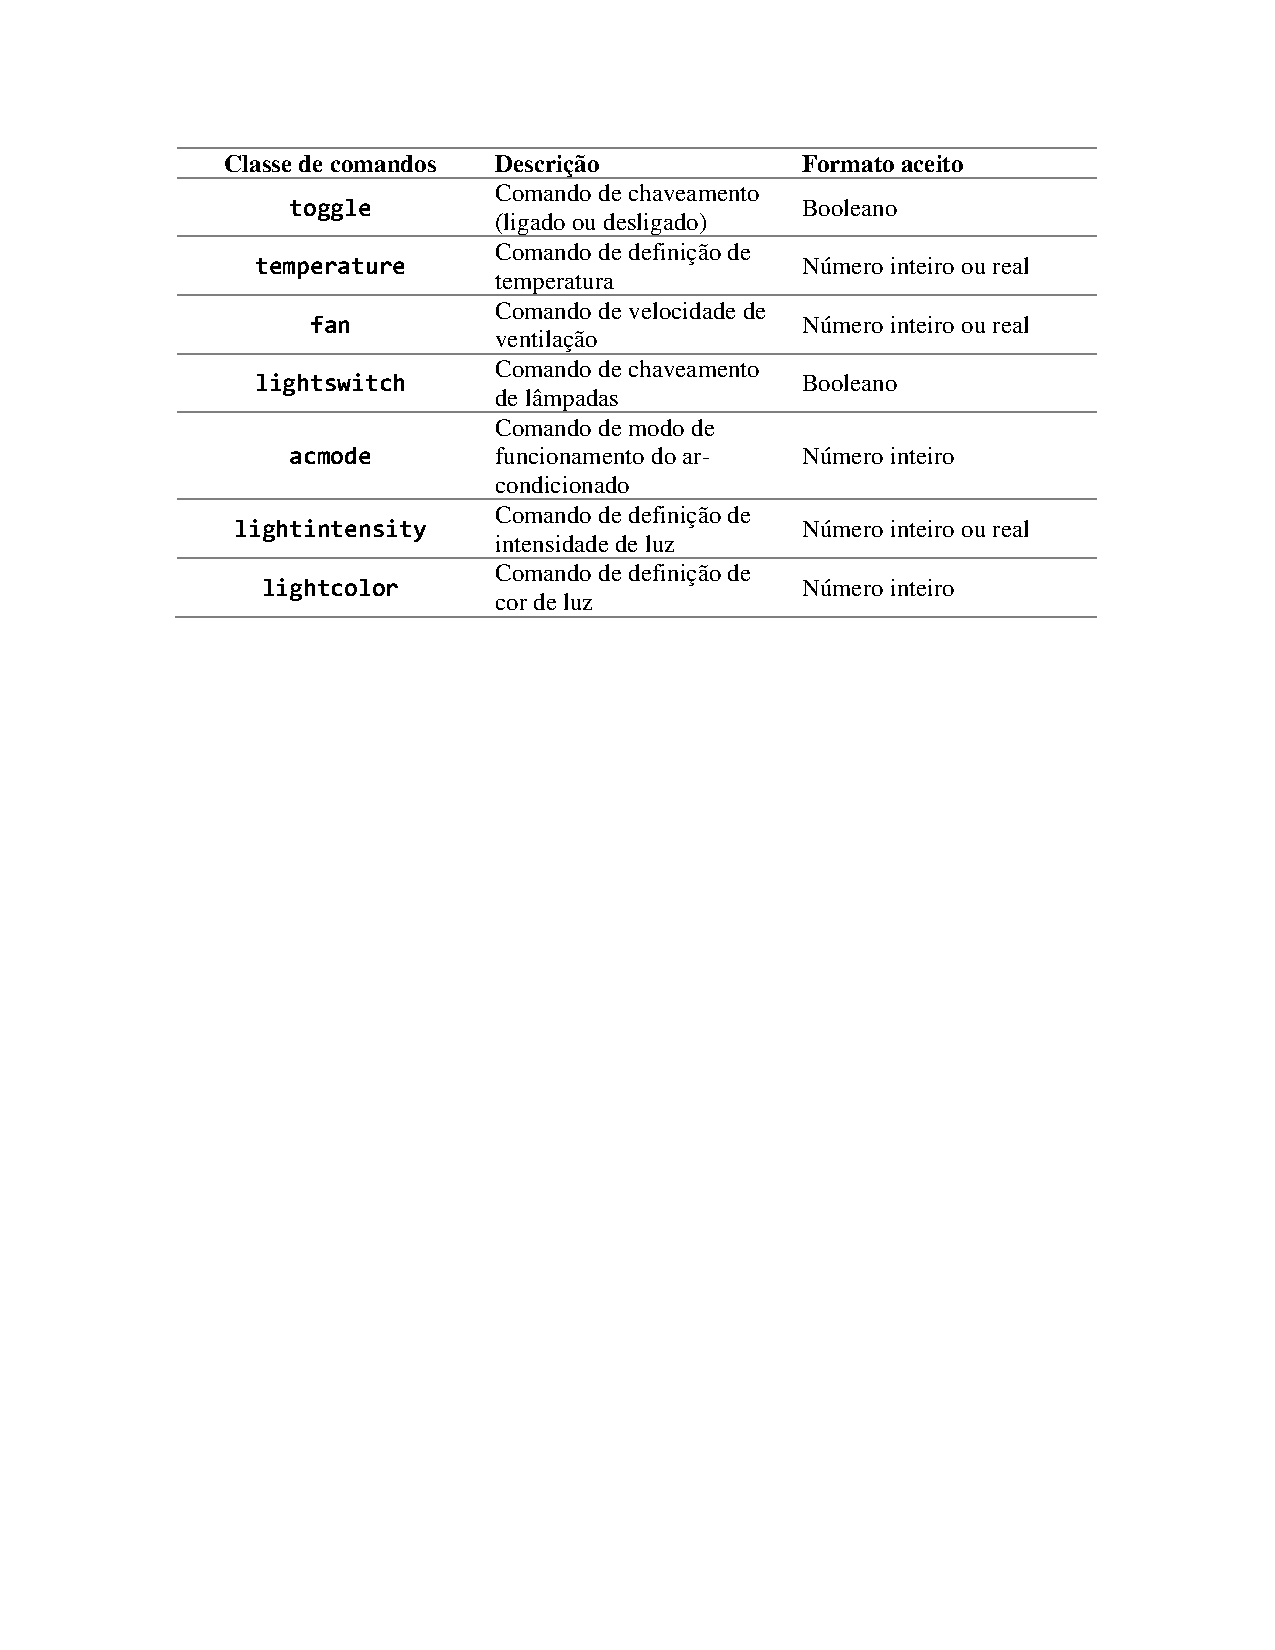
\includegraphics[width=0.9\textwidth]{tabelas/classes_comandos.pdf}
\end{table}

\paragraph*{\texttt{data}.} Descreve uma mensagem contendo dados de leitura de um sensor. Espera-se que um pacote deste tipo conte com o seguinte campo:
\begin{itemize}
	\item \texttt{data}: especifica o dado lido por um sensor. Possui como valor associado um objeto com os campos listados na Tabela \ref{tab:chaves_dado}.
\end{itemize}

\begin{table}[h]
	\centering
	\caption{Chaves e valores associados utilizados na transmissão de um dado por um sensor.}\smallskip
	\label{tab:chaves_dado}
	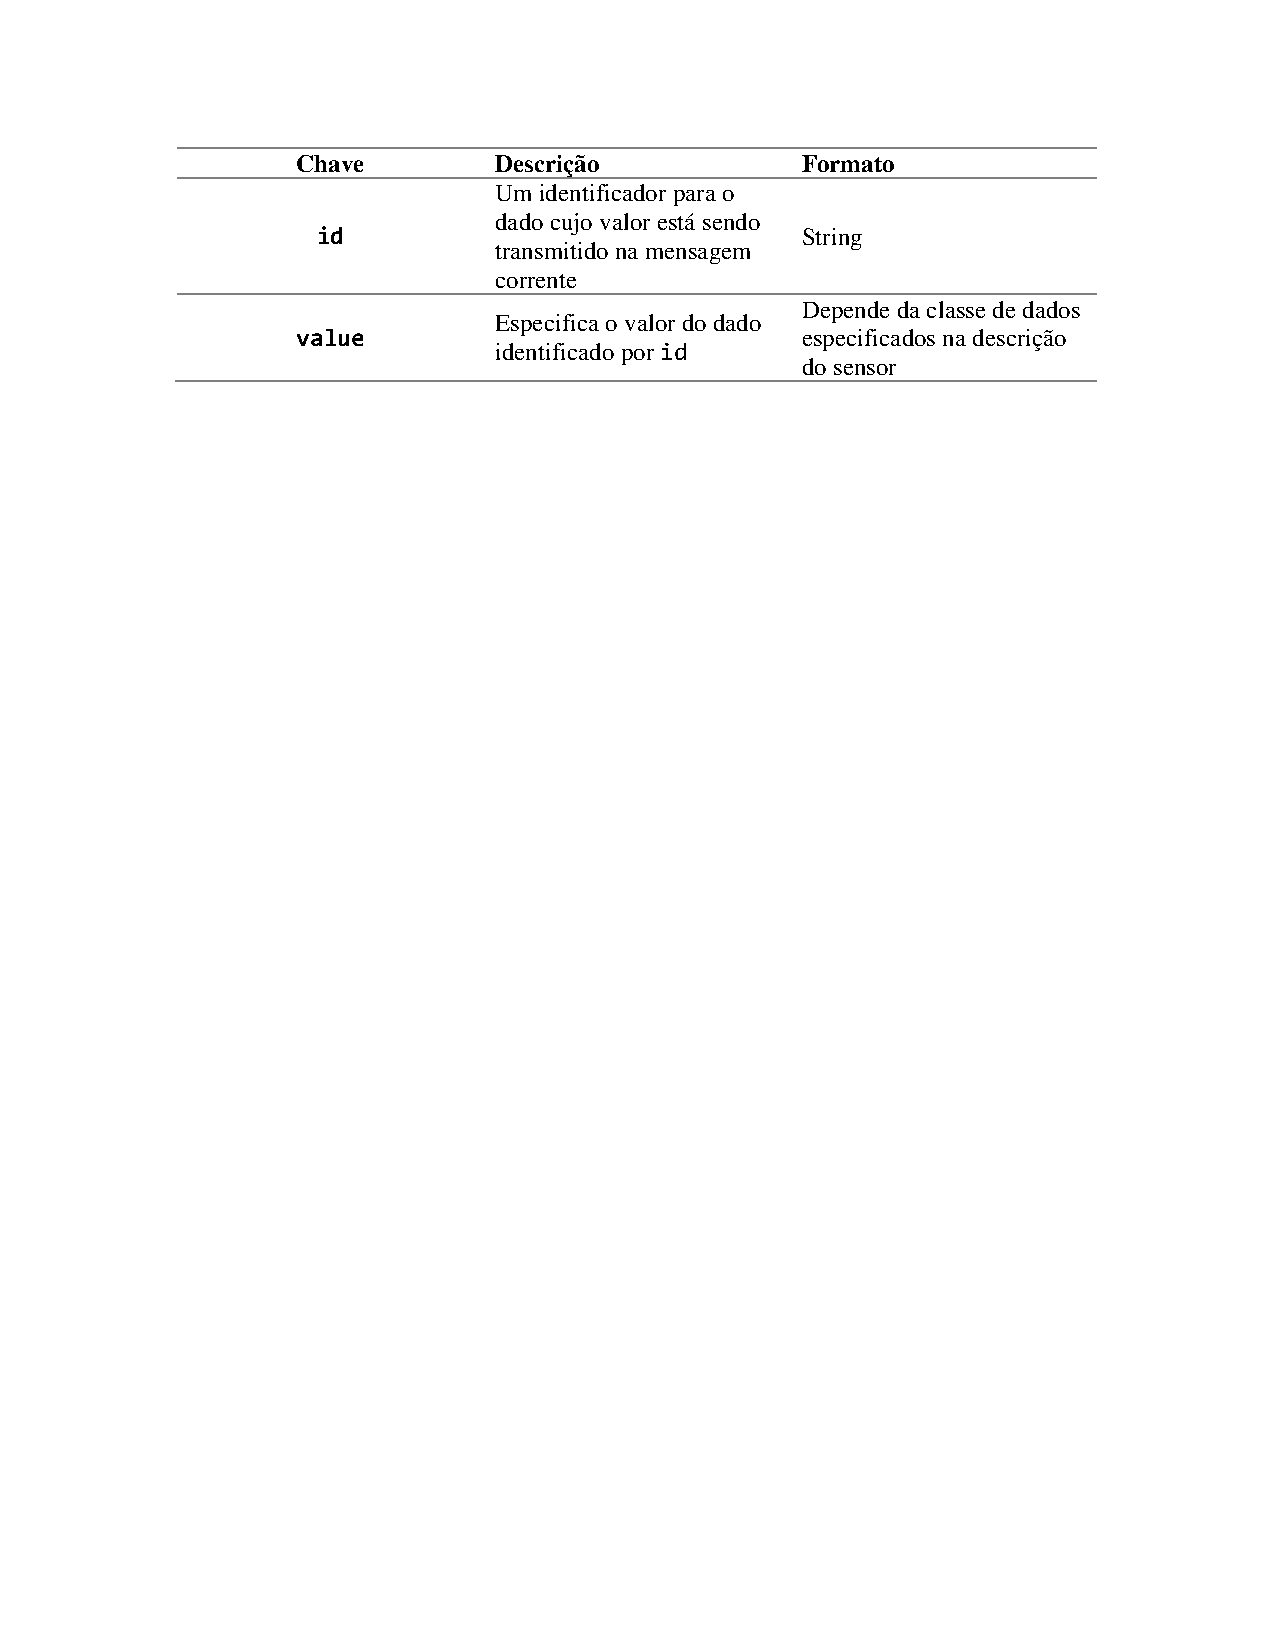
\includegraphics[width=0.9\textwidth]{tabelas/chaves_dado.pdf}
\end{table}

\paragraph*{\texttt{command}.} Descreve uma mensagem contendo comandos destinados a um atuador. Espera-se que um pacote deste tipo conte com o seguinte campo:
\begin{itemize}
	\item \texttt{command} especifica o comando destinado a um atuador. Possui como valor associado um objeto com os campos listados na Tabela \ref{tab:chaves_comando}.
\end{itemize}

\begin{table}[h]
	\centering
	\caption{Chaves e valores associados utilizados na transmissão de um comando para um atuador.}\smallskip
	\label{tab:chaves_comando}
	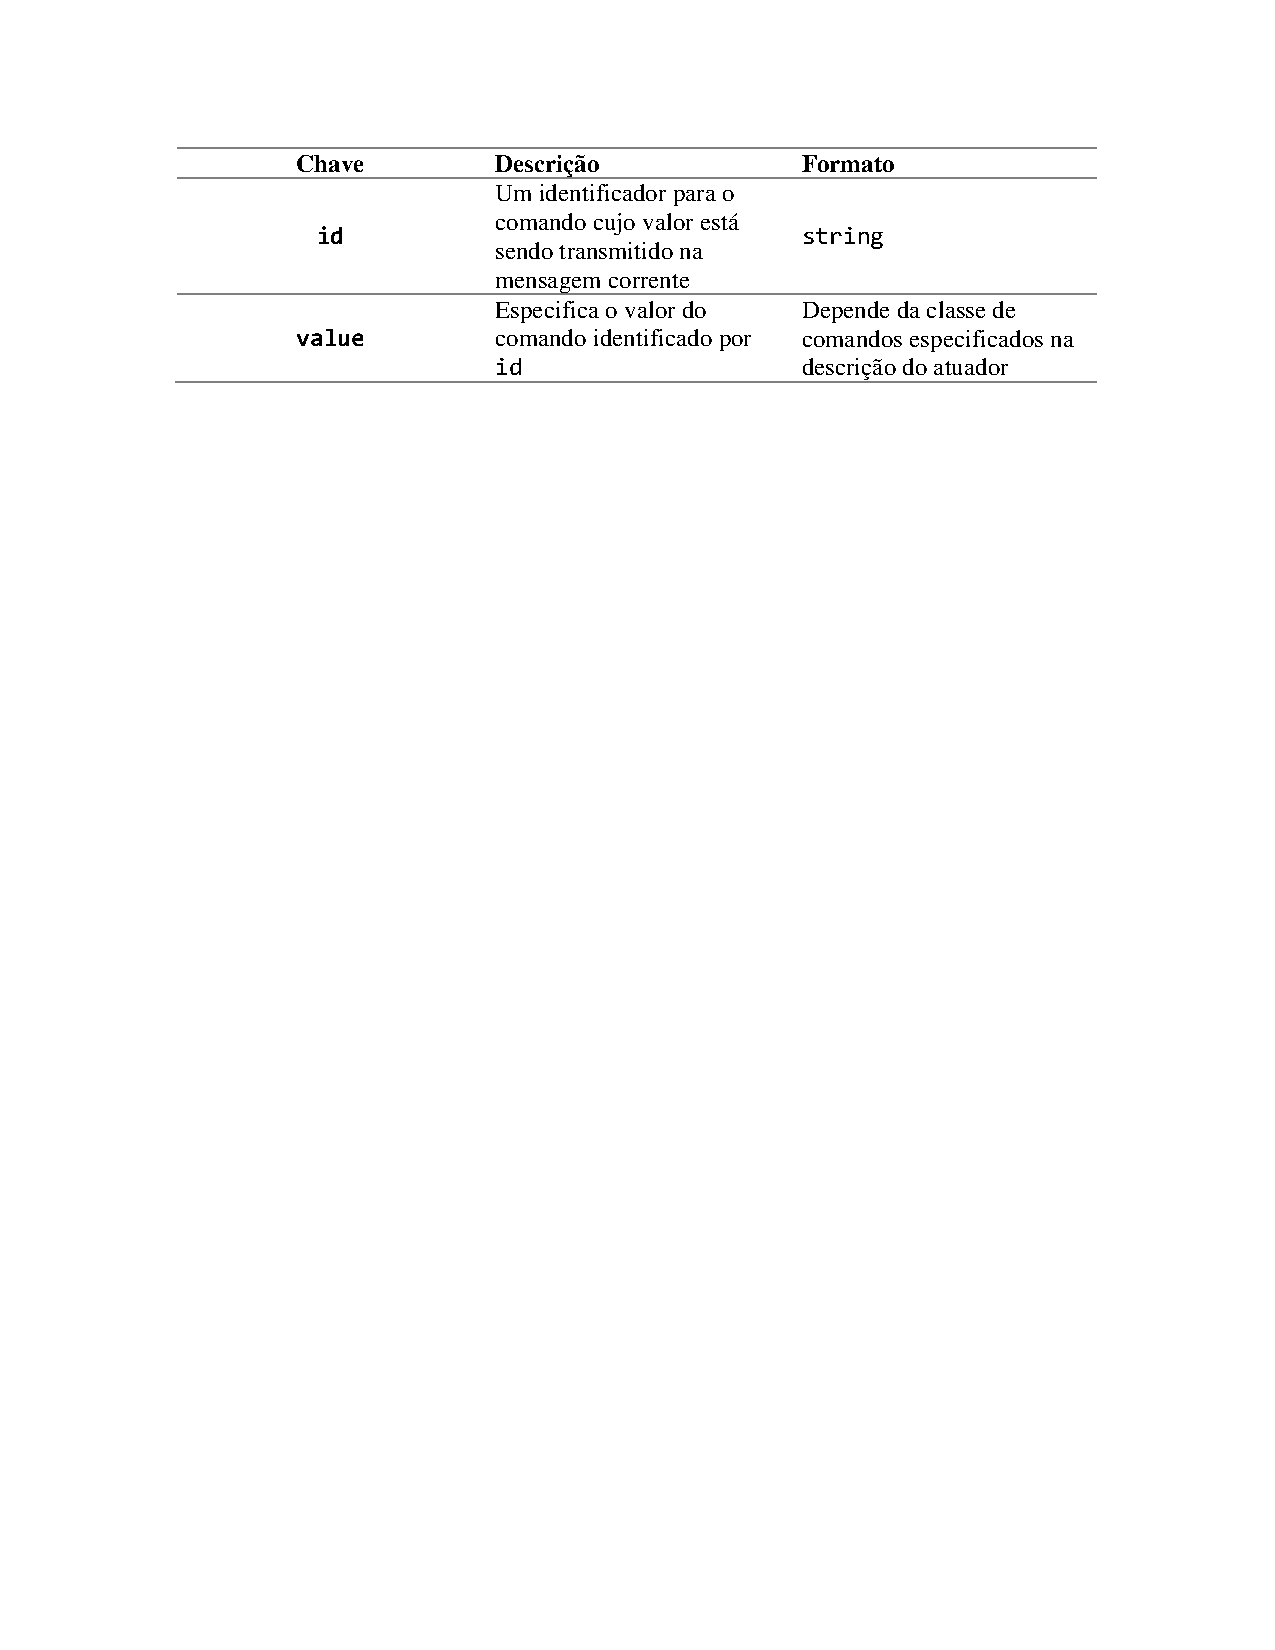
\includegraphics[width=0.9\textwidth]{tabelas/chaves_comando.pdf}
\end{table}

\paragraph*{\texttt{lifetime}.} Mensagem especificando o intervalo máximo de envio de sinais de  \textit{heartbeat}. Espera-se que uma mensagem deste tipo conte com o seguinte campo:
\begin{itemize}
	\item \texttt{lifetime}: especifica o intervalo de tempo máximo entre mensagens de \textit{heartbeat}. Esta mensagem é emitida pelo controlador aos dispositivos, regulando a frequência de envio de mensagens do tipo \texttt{keepalive}.
\end{itemize}

\paragraph*{\texttt{keepalive}.} Especifica uma mensagem que deve ser interpretada como sinal de  \textit{heartbeat}.

\paragraph*{\texttt{iamback}.} Emitida por um sensor ou atuador caso ele tenha recebido um identificador anteriormente, mas devido a alguma razão, foi desconectado da rede e necessita se reconectar.

\paragraph*{\texttt{welcomeback}.} Mensagem emitida por um controlador ao receber uma mensagem do tipo \texttt{iamback}, indicando que o dispositivo foi reconhecido e aceito na rede.

\paragraph*{\texttt{externalcommand}.} Mensagem emitida por um dispositivo atuador, indicando que um comando de origem externa ao sistema foi recebido. A estrutura desta mensagem é igual às do tipo \texttt{command}.

Cabe apontar que as mensagens dos tipos \texttt{description}, \texttt{data}, \texttt{command}, \texttt{keepalive}, \texttt{iamback} e \texttt{externalcommand} devem possuir o campo \texttt{id}, que identifica o dispositivo.

Note, ainda, que chaves do tipo \texttt{packageType} e \texttt{nodeClass} podem ter múltiplos valores associados. Por exemplo, uma mensagem pode ser enviada com os tipos \texttt{iamcontroller}, \texttt{describeyourself} e \texttt{lifetime}, indicando que ela tem as funções de identificar o controlador, solicitar informações ao dispositivo-destino e definir o intervalo de envio de sinais de \textit{heartbeat}.

\subsection{Protocolo de Troca de Mensagens}
Definida a estrutura do pacote, suas chaves e seus valores associados, pode-se passar para a definição do aspecto dinâmico do protocolo. Esta seção busca definir o sequenciamento de mensagens para efetuar ações específicas na rede de sensores.

\paragraph*{Inicialização.} O processo de inicialização dos sensores está esquematizado na Figura \ref{fig:uml_handshake}. Assim que um dispositivo é conectado à rede, ele emite um pacote do tipo \texttt{whiiscontroller} em \textit{broadcast}, com o objetivo de descobrir o endereço do controlador, caso exista. Em seguida, o controlador responde com uma mensagem do tipo \texttt{iamcontroller} ao dispositivo solicitante, permitindo que ele identifique o endereço do coordenador. Além disso, nesta mensagem, o controlador define o identificador do dispositivo.

Em seguida, o controlador solicita uma descrição do dispositivo com um pacote do tipo \texttt{describeyourself}, ao qual o dispositivo responde com uma mensagem \texttt{description}. Ela contém informações como a classe do nó, tipos de dados gerados (caso seja sensor) e tipos de comandos aceitos (caso seja atuador).

O controlador também pode definir um intervalo máximo em que o dispositivo deve enviar mensagens de \textit{heartbeat} através do pacote \texttt{lifetime}. O dispositivo, neste caso, envia pacotes \textit{heartbeat} periodicamente, sinalizando os pacotes como sendo do tipo \texttt{keepalive}.

\begin{figure}[h]
	\centering

	\caption{Processo de inicialização de um dispositivo.} 
	\medskip
  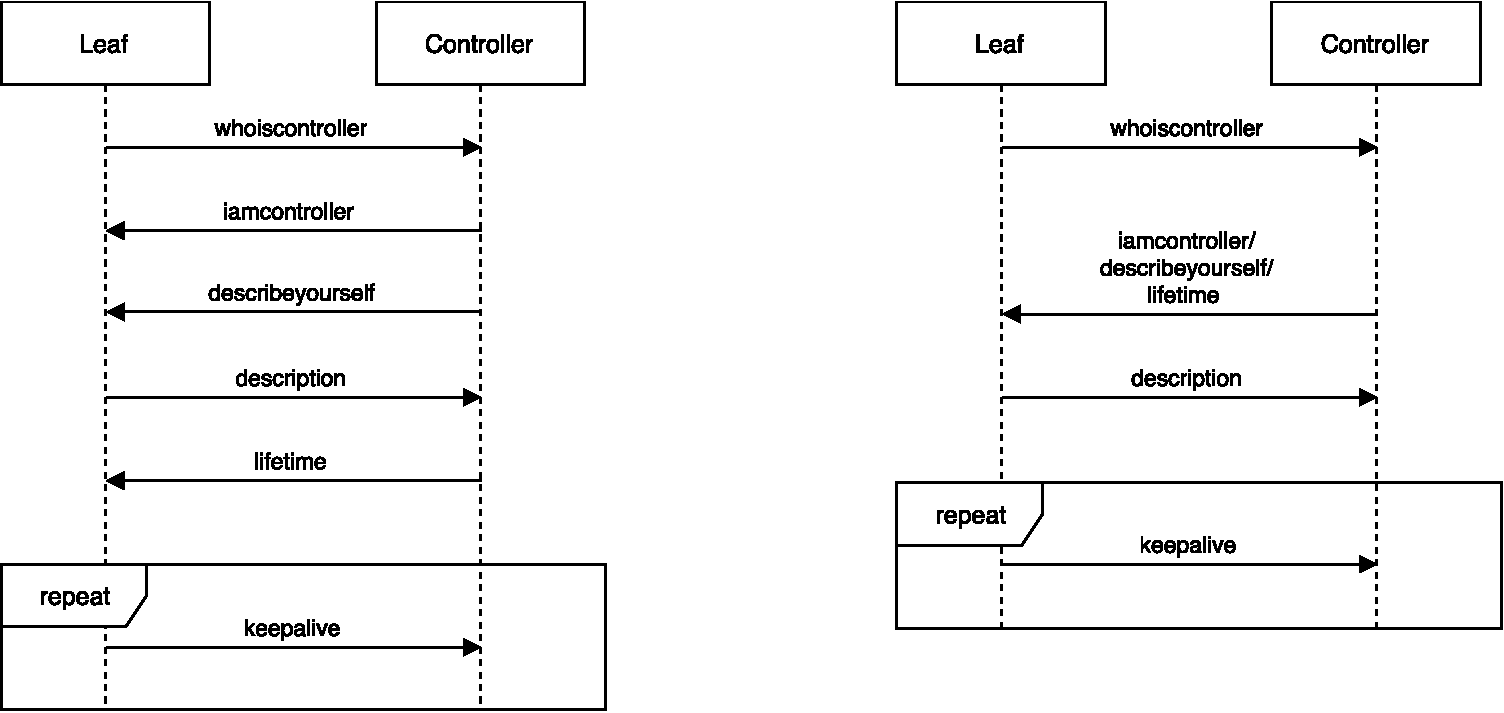
\includegraphics[width=\textwidth]{imagens/uml_handshake.pdf}
  \label{fig:uml_handshake}
\end{figure}

O processo de inicialização pode ser simplificado condensando-se os pacotes \texttt{iamcontroller}, \texttt{describeyourself} e \texttt{lifetime} (caso aplicável) em um único pacote, conforme ilustra o diagrama à direita da Figura \ref{fig:uml_handshake}.

\paragraph*{Envio de dados.} Uma vez efetuado o processo de inicialização, dados de leitura podem ser enviados do sensor ao controlador através da mensagem \texttt{data}.

\paragraph*{Envio de comandos.} Uma vez efetuado o processo de inicialização, comandos podem ser enviados do controlador ao atuador através da mensagem \texttt{command}.

\paragraph*{Retorno à rede.} Caso um dispositivo operante se desconecte da rede por algum motivo, ele pode se reconectar enviando uma mensagem do tipo \texttt{imback}, conforme ilustra a Figura \ref{fig:uml_reconnect}. Ao receber uma mensagem deste tipo, o controlador pode responder de duas maneiras. Caso ele reconheça o identificador enviado pelo dispositivo na mensagem \texttt{imback}, ele responde com outra mensagem do tipo \texttt{welcomeback}, conforme ilustra o diagrama à esquerda da Figura \ref{fig:uml_reconnect}. A partir deste momento, o dispositivo pode operar regularmente. Por outro lado, caso o controlador não reconheça o dispositivo, ele solicita uma nova declaração, como ilustrado no diagrama à direita da Figura \ref{fig:uml_reconnect}.

\begin{figure}[h]
	\centering
	\caption{Processo de retorno de um dispositivo à rede.}
	\medskip
  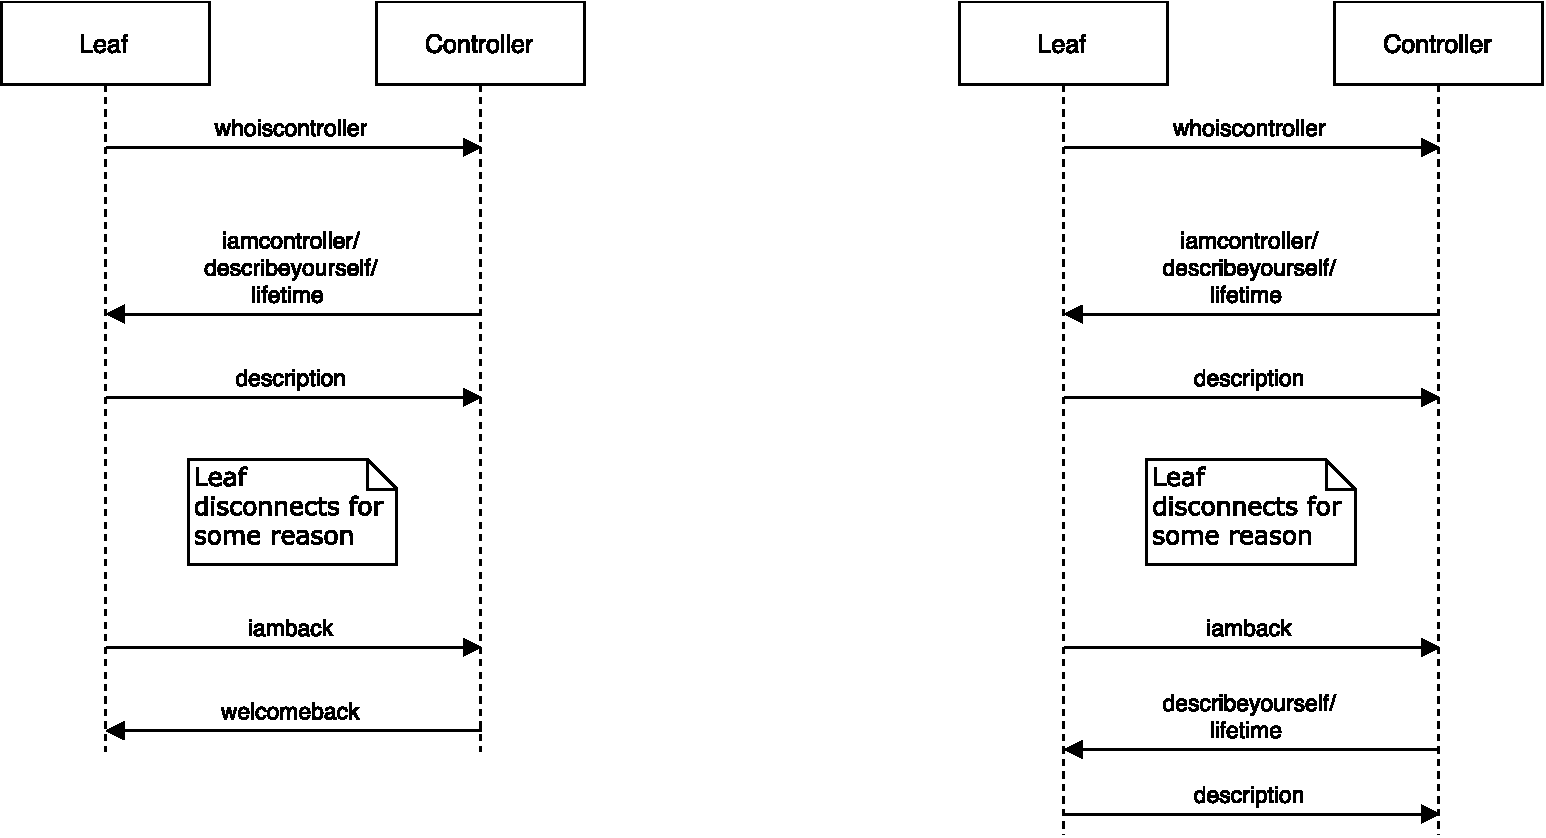
\includegraphics[width=\textwidth]{imagens/uml_reconnect.pdf}
  \label{fig:uml_reconnect}
\end{figure}

\subsection{A codificação CBOR}
Como mencionado, redes de sensores sem fio são compostas por dispositivos com limitações de banda e de processamento. Por esta razão, é importante que as mensagens trafegadas sejam concisas (aliviando requisitos de banda) e de simples interpretação (aliviando requisitos de processamento). Com esses propósitos em mente, resolveu-se adotar a codificação CBOR (\textit{Concise Binary Object Representation}) \cite{rfc7049}.

Esta codificação é baseada no formato de dados JSON, provendo uma maneira de representar objetos neste formato de forma binária. Sua especificação reconhece diversos tipos de dados, tais como inteiros negativos e não-negativos, cadeias de bytes e de caracteres, entre outros, cada qual com regras específicas de representação. Para identificar o tipo de cada dado, a codificação dedica um byte para cada item de dado para descrevê-lo.

Considere como exemplo a codificação do objeto JSON a seguir:
\begin{center}
	\texttt{\{"a": 1, "b": 2\}}
\end{center}

Uma representação possível do objeto acima pode ser feito em forma de cadeia de caracteres. Apresar de ser uma forma comum e prática de se representar tais objetos, ela possui a desvantagem de ser extensa: no exemplo dado, considerando que um caractere ocupa 1 byte, o resultado gerado possui 13 bytes. Por outro lado, sua representação em CBOR ocupa 7 bytes, conforme apresentado na Tabela \ref{tab:cbor_exemplo}. Isso corresponde a uma redução de quase 50\% no resultado gerado.

\begin{table}[h]
	\centering
	\caption{Exemplo de representação em CBOR de um objeto JSON.}\smallskip
	\label{tab:cbor_exemplo}
	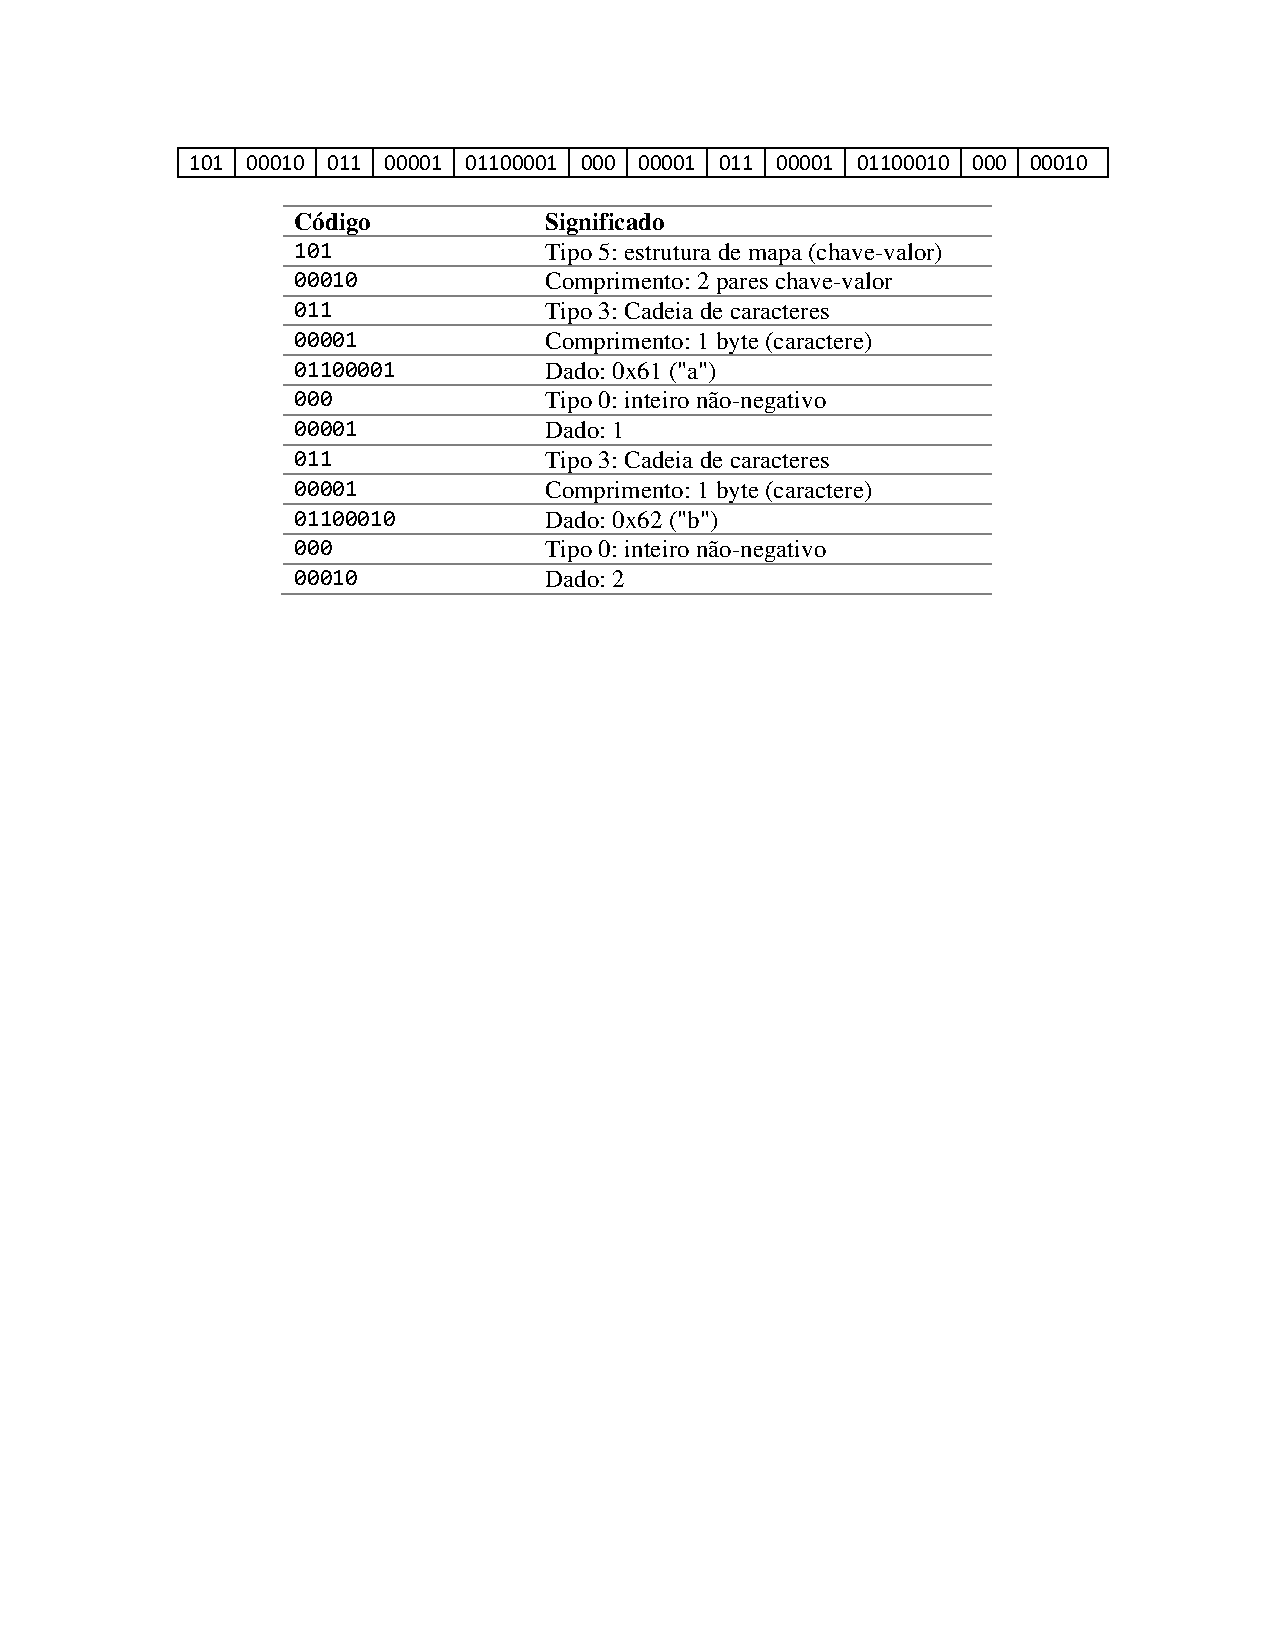
\includegraphics[width=0.9\textwidth]{tabelas/cbor_exemplo.pdf}
\end{table}

\subsection{Codificação dos Itens nas Mensagens}
Seguindo a ideia de manter concisão nas mensagens trocadas, e levando em conta o funcionamento da codificação CBOR, os campos e valores especificados na seção \ref{subsec:sintaxe} devem ser codificados antes da transmissão. As Tabelas \ref{tab:codificacao_chaves_principais}, \ref{tab:codificacao_tipo_dc} e \ref{tab:codificacao_dc} listam as codificações adotadas para as chaves das mensagens transmitidas.

\begin{table}[hp]
	\centering
	\caption{Codificação das chaves principais de uma mensagem.}\smallskip
	\label{tab:codificacao_chaves_principais}
	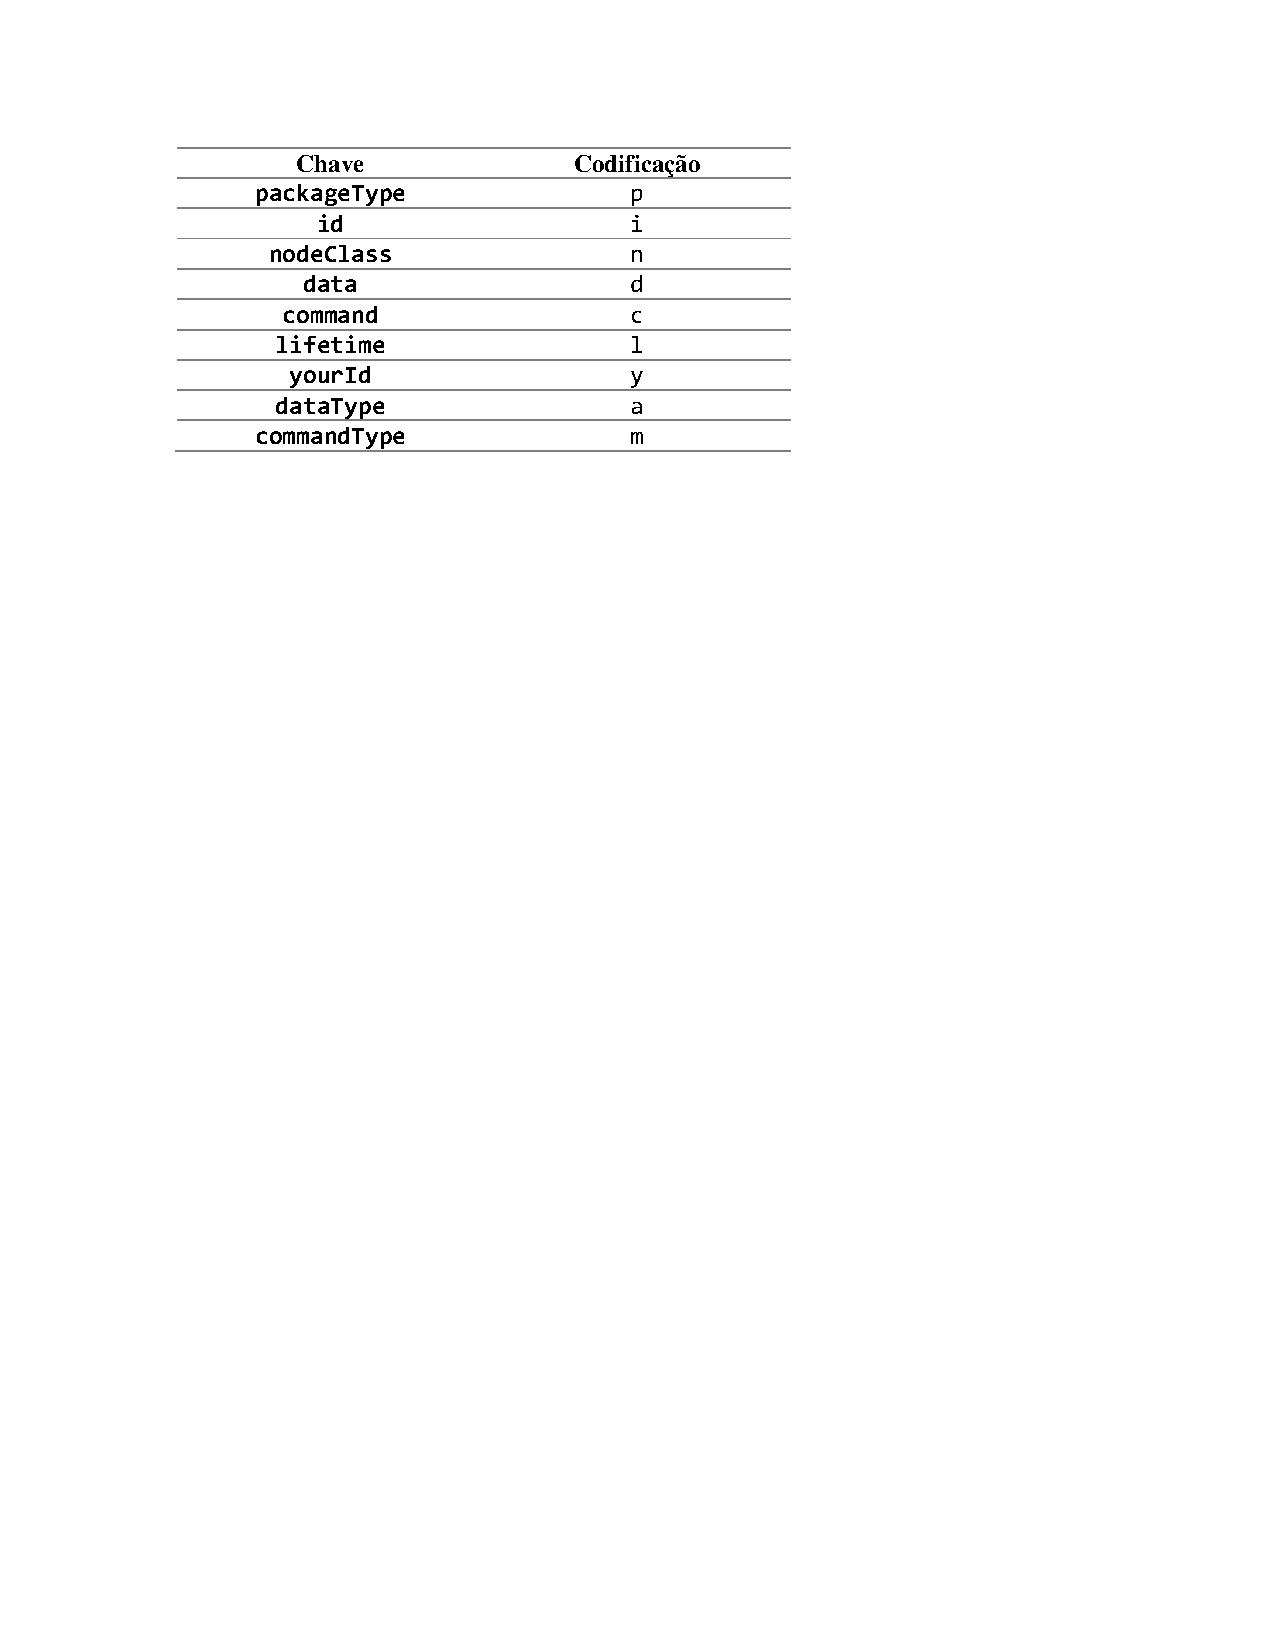
\includegraphics[width=0.7\textwidth]{tabelas/codificacao_chaves_principais.pdf}
	
	\caption{Codificação de chaves utilizadas nos campos \texttt{datatype} e \texttt{commandtype}.}\smallskip
	\label{tab:codificacao_tipo_dc}
	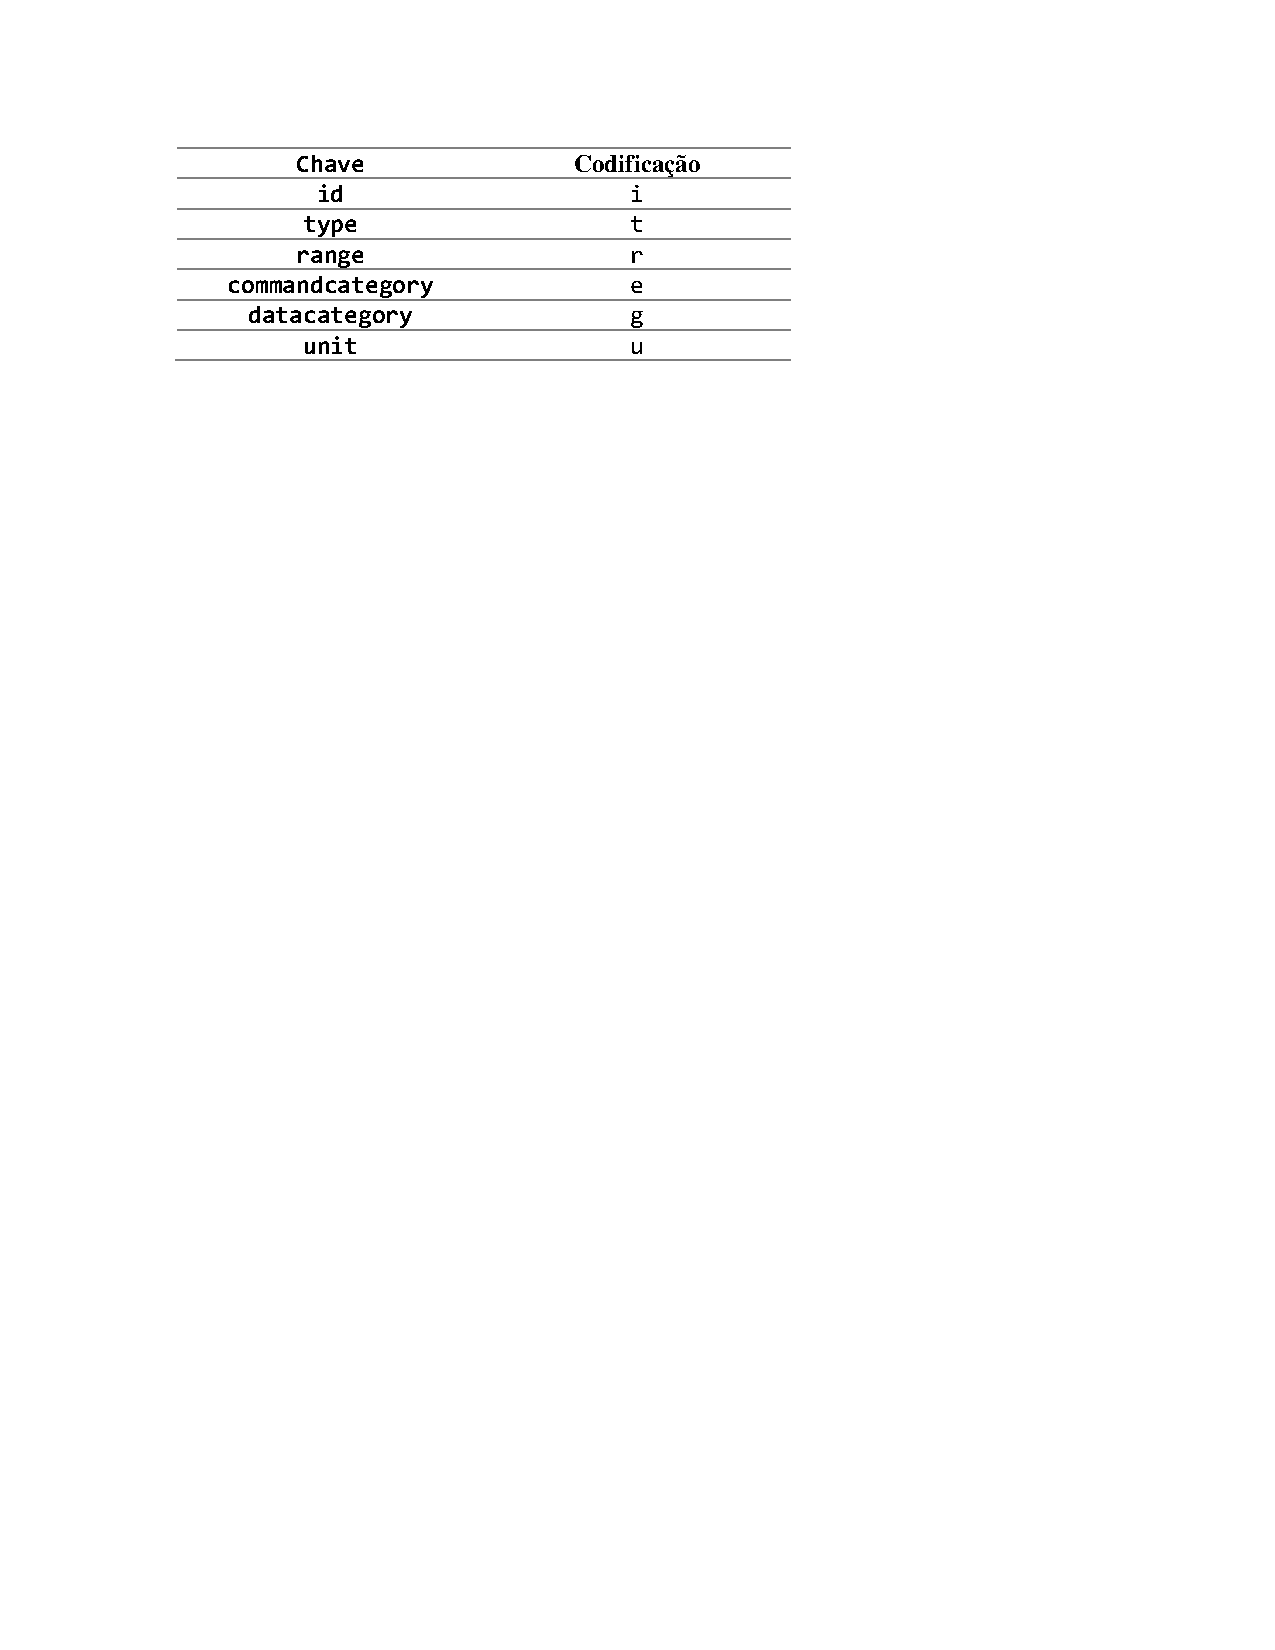
\includegraphics[width=0.7\textwidth]{tabelas/codificacao_tipo_dc.pdf}
	
	\caption{Codificação de chaves utilizadas em mensagens do tipo \texttt{data} e \texttt{command}.}\smallskip
	\label{tab:codificacao_dc}
	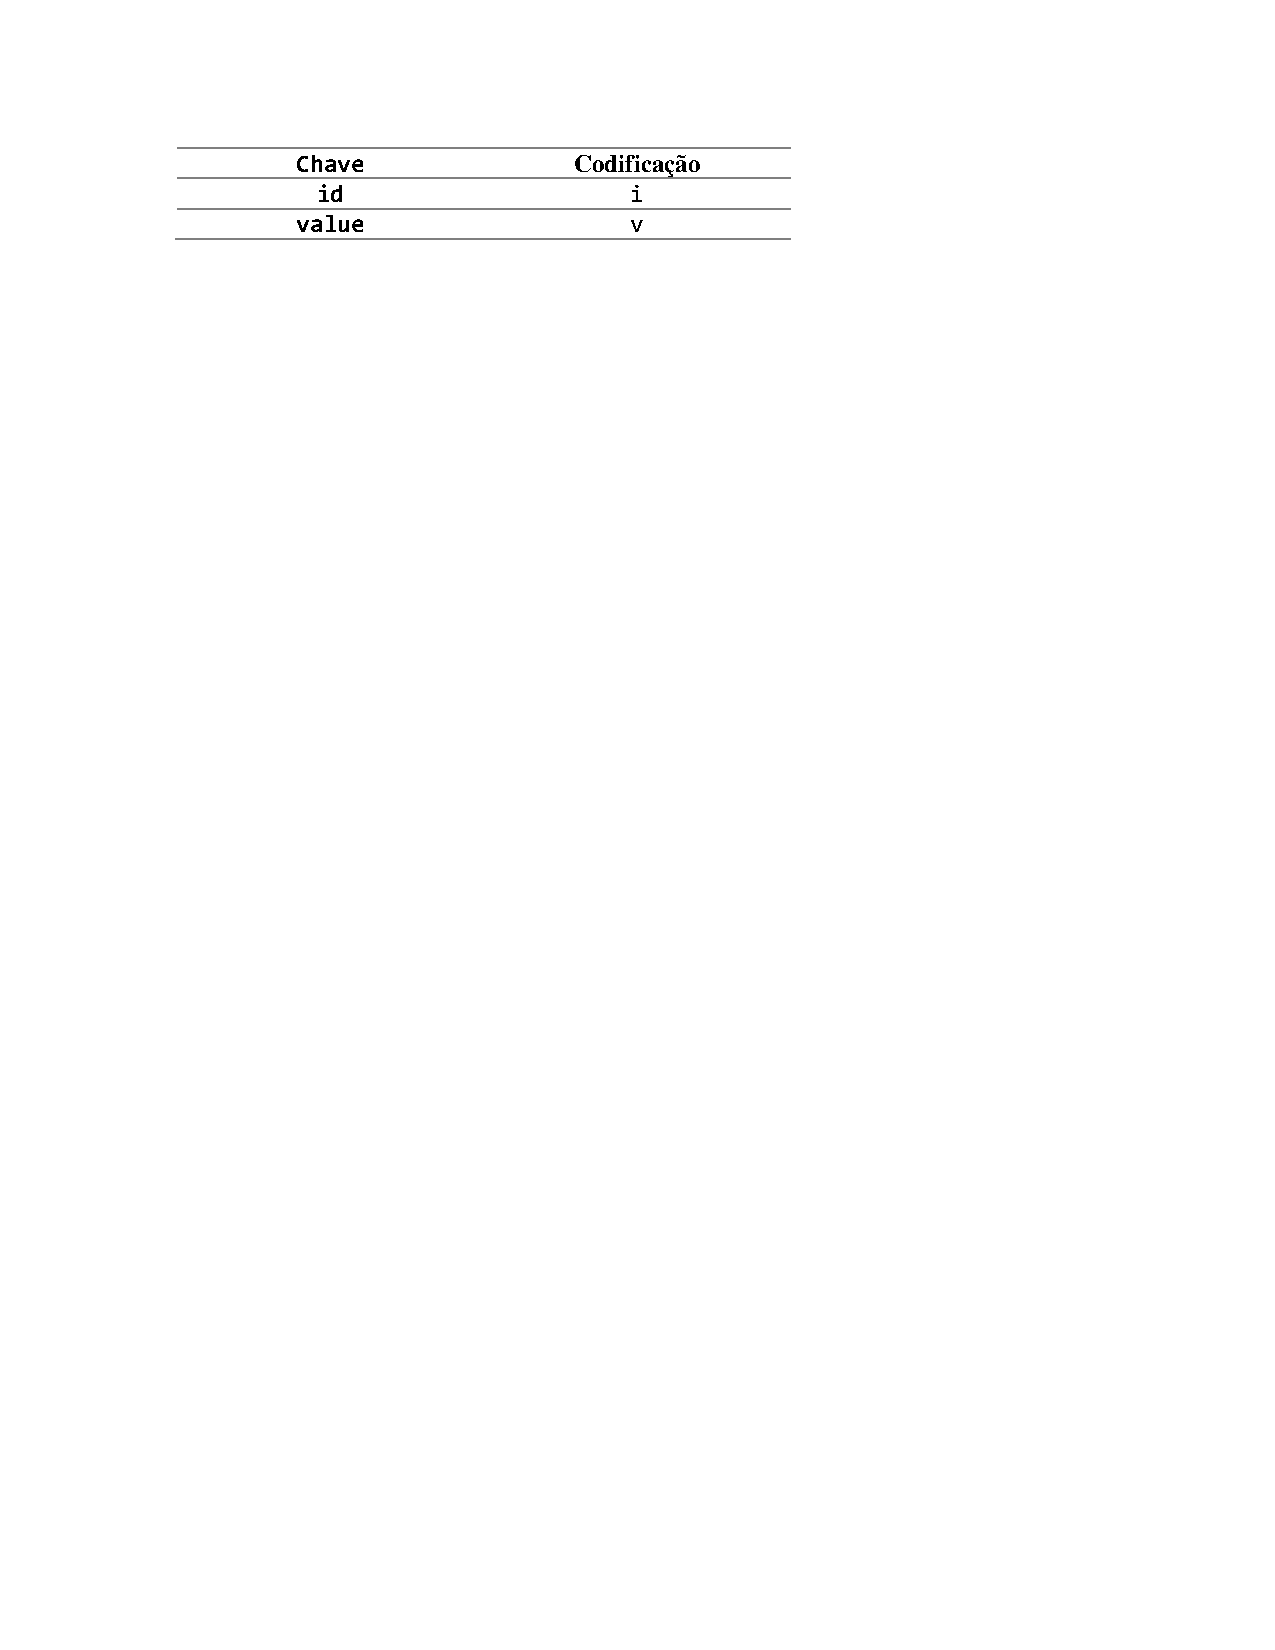
\includegraphics[width=0.7\textwidth]{tabelas/codificacao_dc.pdf}
	
\end{table}

De modo similar, as Tabelas \ref{tab:cod_valores_packagetype}, \ref{tab:cod_valores_nodeclass}, \ref{tab:cod_valores_measurestrat}, \ref{tab:cod_data_category}, \ref{tab:cod_command_category} e \ref{tab:cod_type_category} listam as codificações adotadas para os valores utilizados em diversos campos das mensagens. Observe que os valores utilizados nos campos \texttt{packageType} (Tabela \ref{tab:cod_valores_packagetype}) e \texttt{nodeClass} (Tabela \ref{tab:cod_valores_nodeclass}) evoluem em potências de 2. Isso ocorre pois, conforme apontado na seção \ref{subsec:sintaxe}, tais campos permitem múltiplos valores. Deste modo, a representação de mais de um valor é feita efetuando-se uma operação de OR binário. Por exemplo, se um dado dispositivo for tanto sensor (código 1) quanto atuador (código 2), sua representação se dará enviando um pacote contendo o campo \texttt{nodeClass} definido para 3.

\begin{table}[hp]
	\centering
	\caption{Codificação dos valores do campo \texttt{packageType}.}\smallskip
	\label{tab:cod_valores_packagetype}
	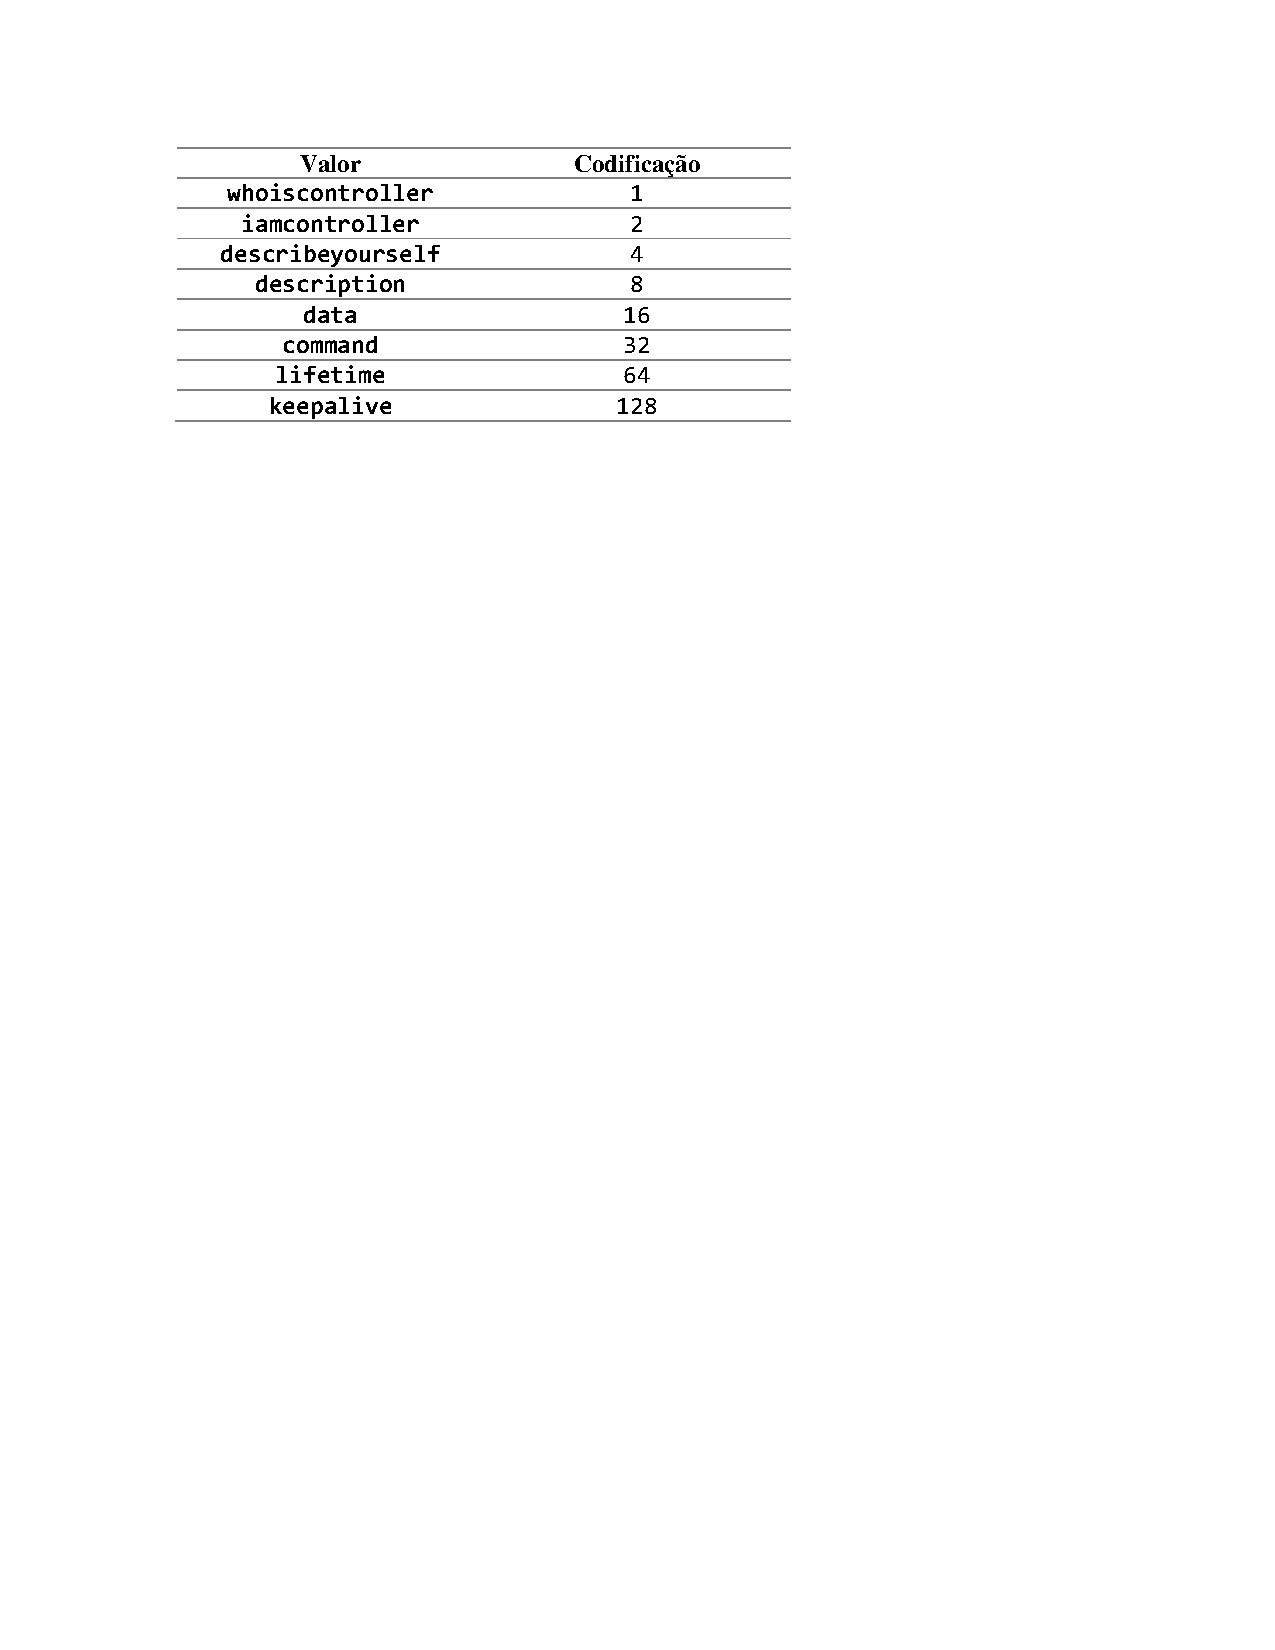
\includegraphics[width=0.7\textwidth]{tabelas/cod_valores_packagetype.pdf}
\end{table}

\begin{table}[hp]	
	\centering
	\caption{Codificação de valores do campo \texttt{nodeClass}.}\smallskip
	\label{tab:cod_valores_nodeclass}
	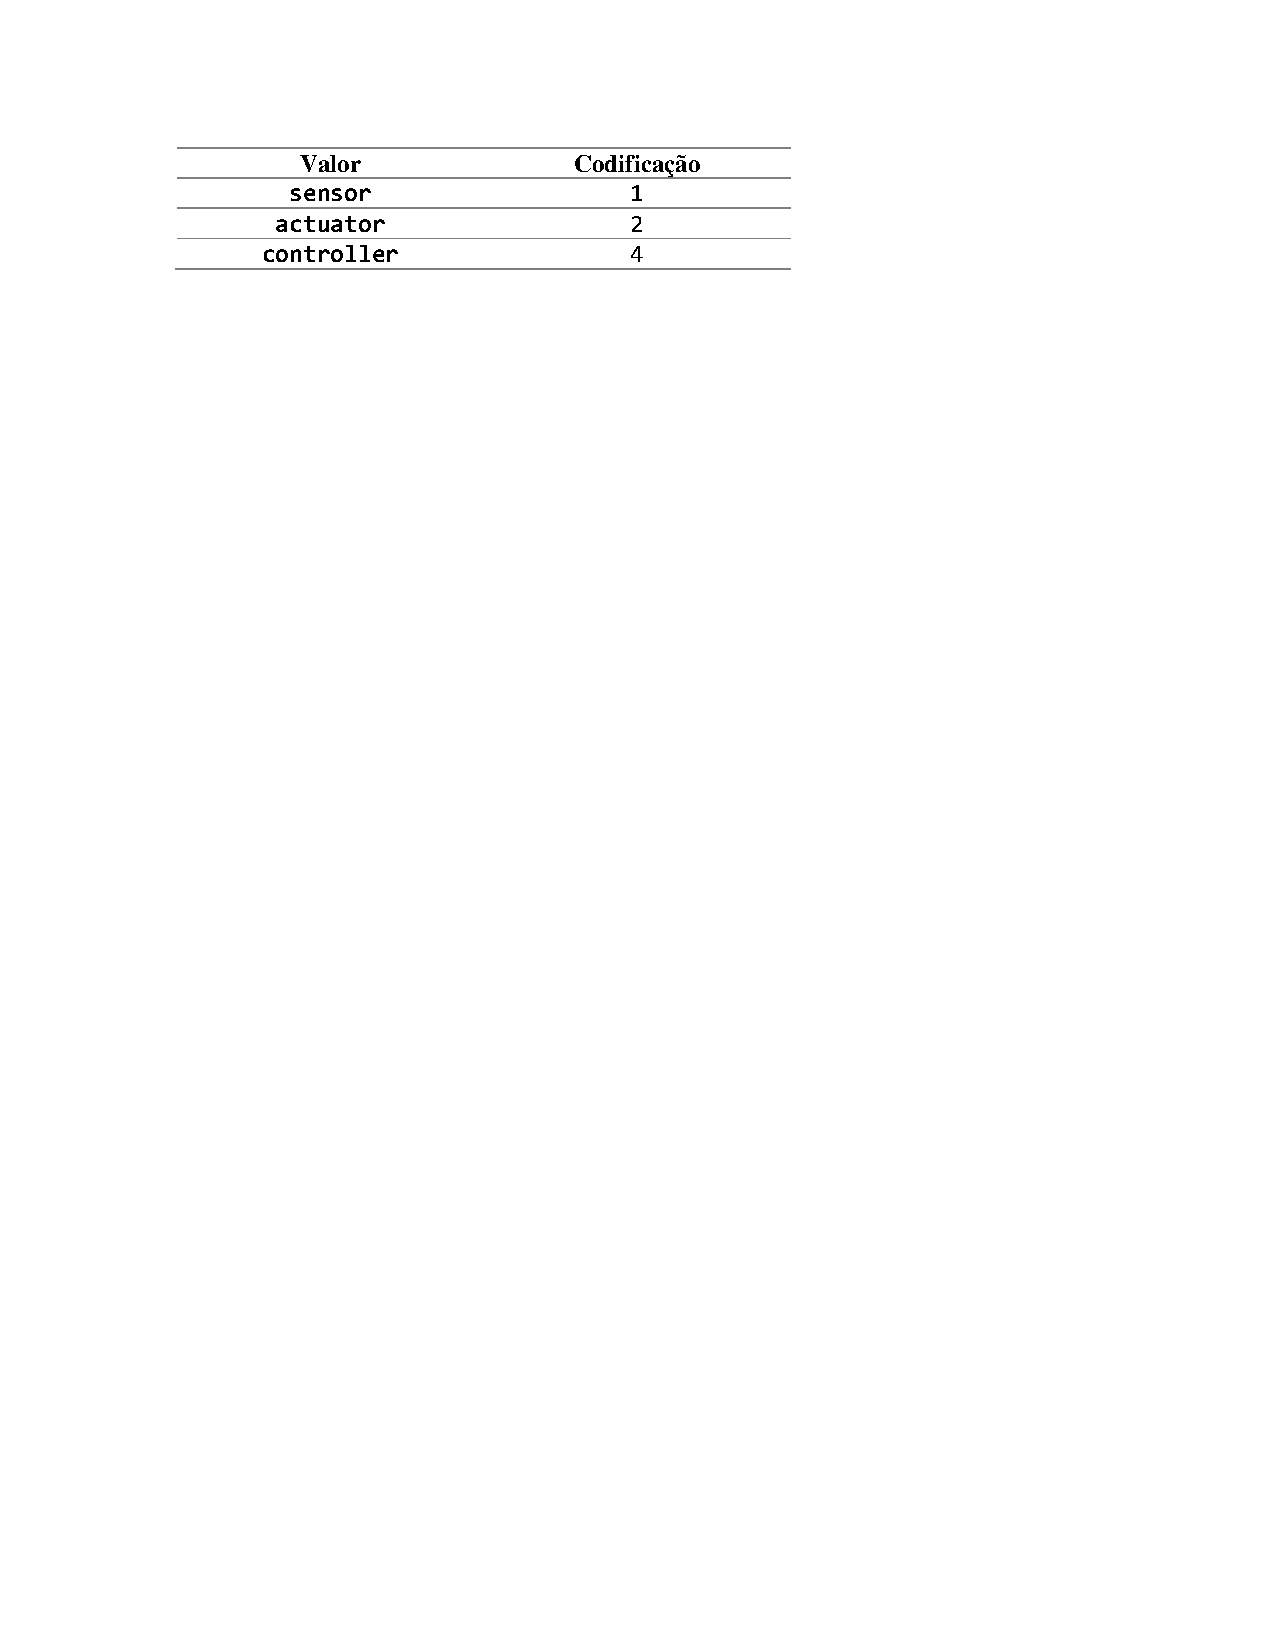
\includegraphics[width=0.7\textwidth]{tabelas/cod_valores_nodeclass.pdf}
\end{table}

\begin{table}[hp]	
	\centering
	\caption{Codificação de valores do campo \texttt{measureStrategy}.}\smallskip
	\label{tab:cod_valores_measurestrat}
	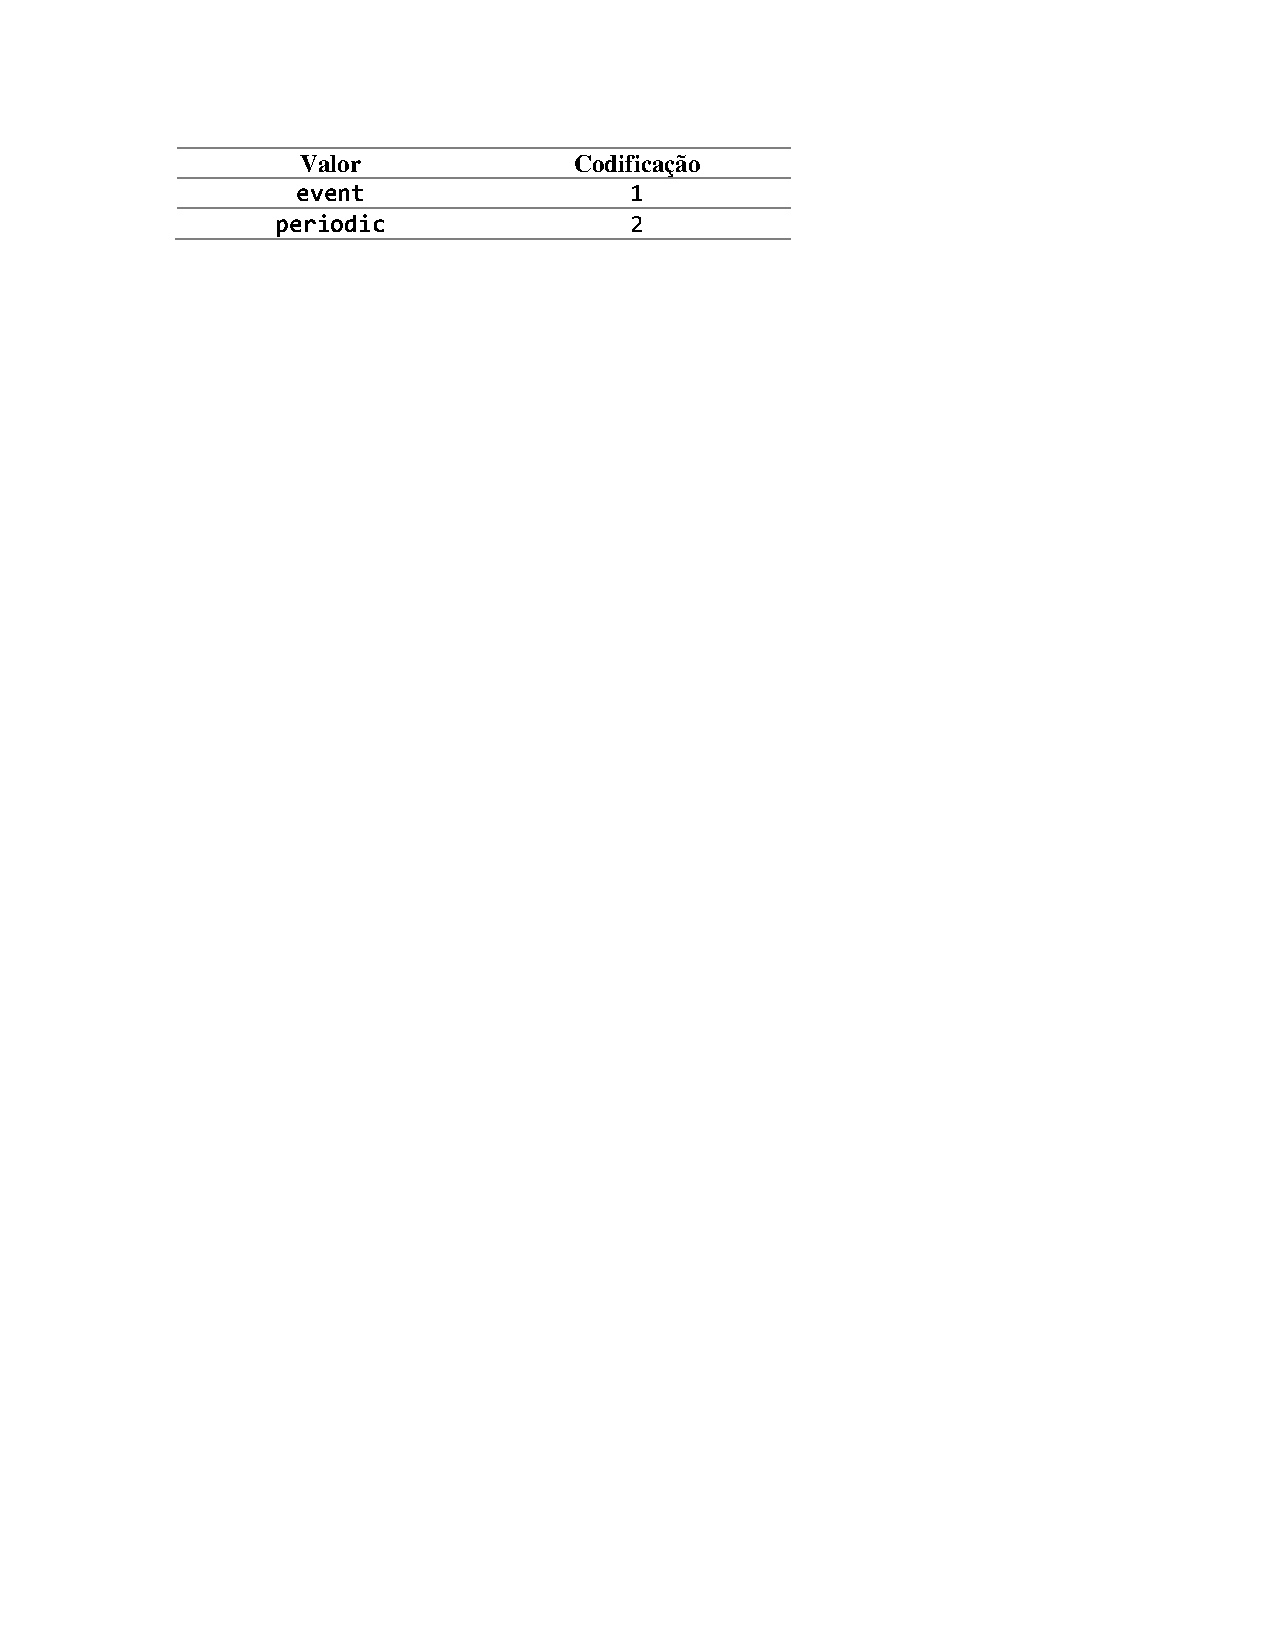
\includegraphics[width=0.7\textwidth]{tabelas/cod_valores_measurestrat.pdf}
\end{table}

\begin{table}[hp]	
	\centering
	\caption{Codificação de valores de categoria para sensores}\smallskip
	\label{tab:cod_data_category}
	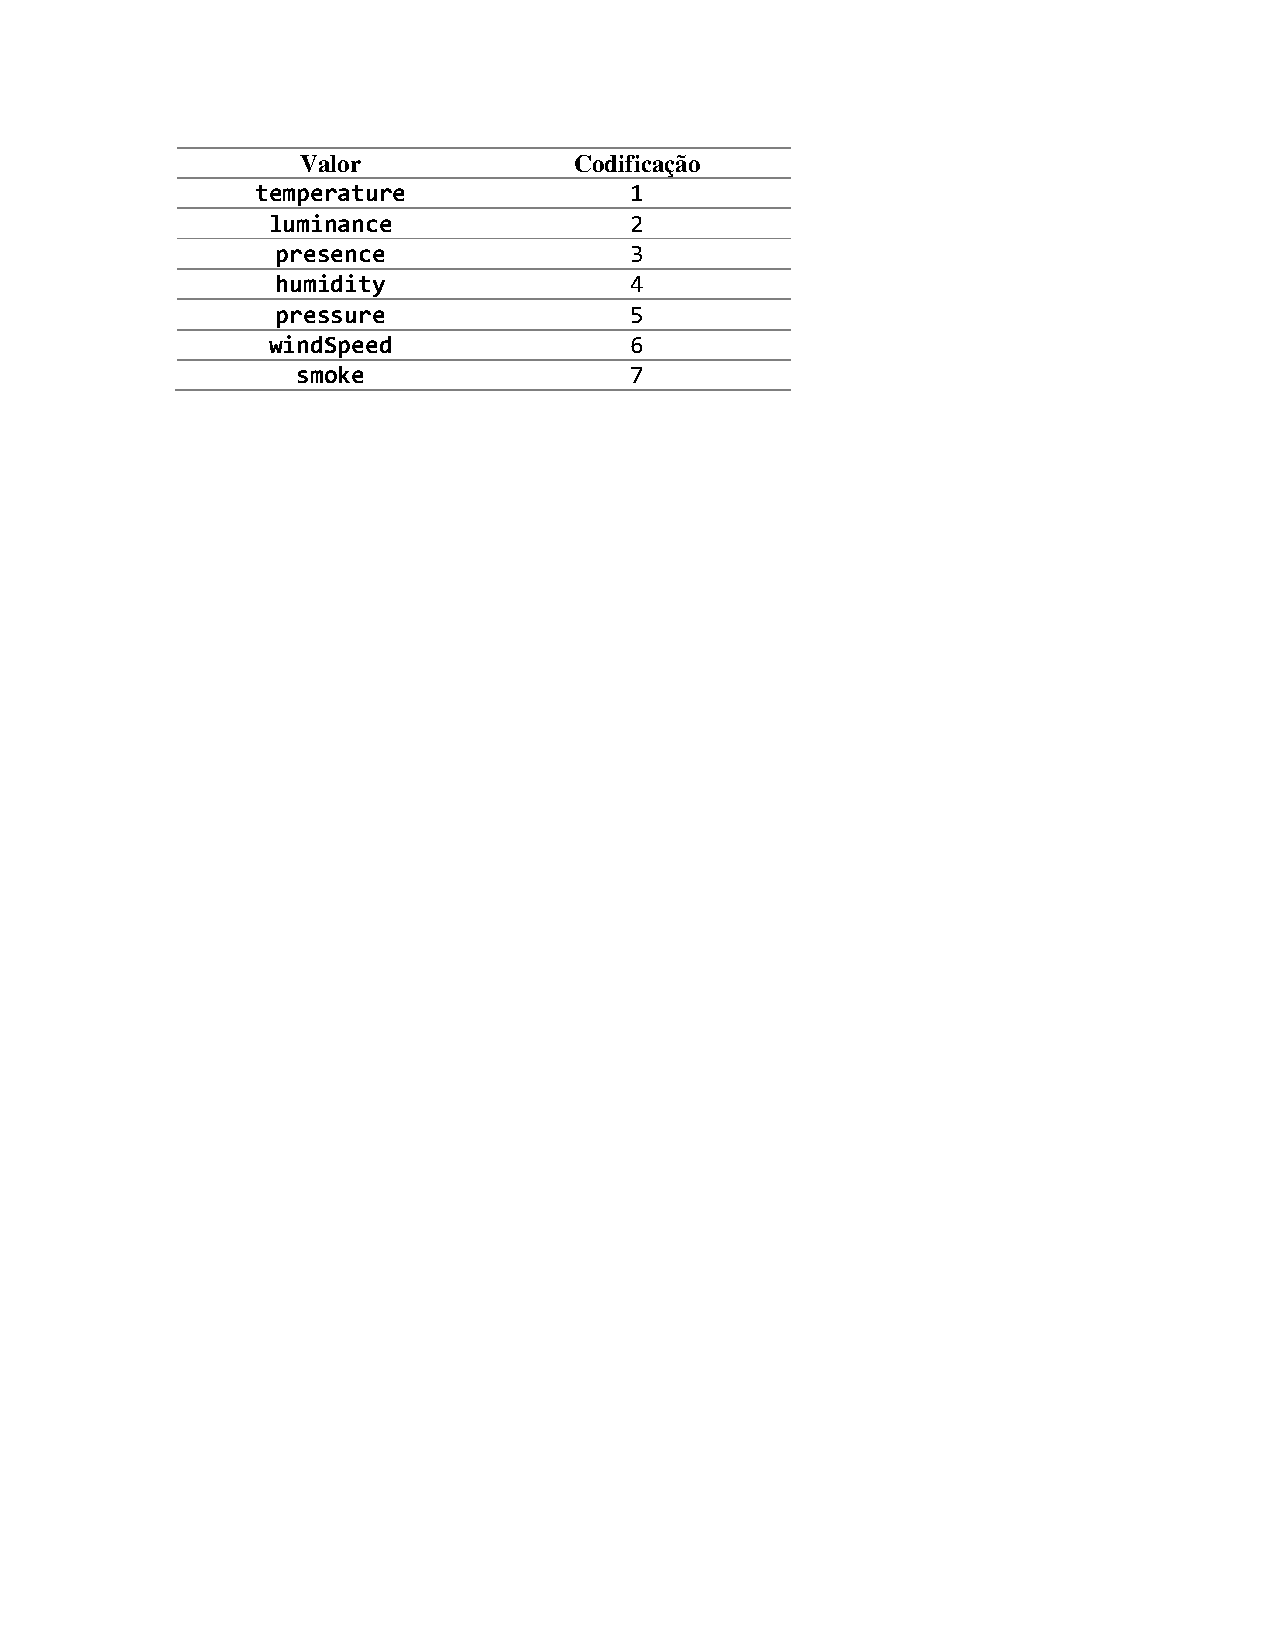
\includegraphics[width=0.7\textwidth]{tabelas/cod_data_category.pdf}
\end{table}

\begin{table}[hp]	
	\centering
	\caption{Codificação de valores de categoria para atuadores}\smallskip
	\label{tab:cod_command_category}
	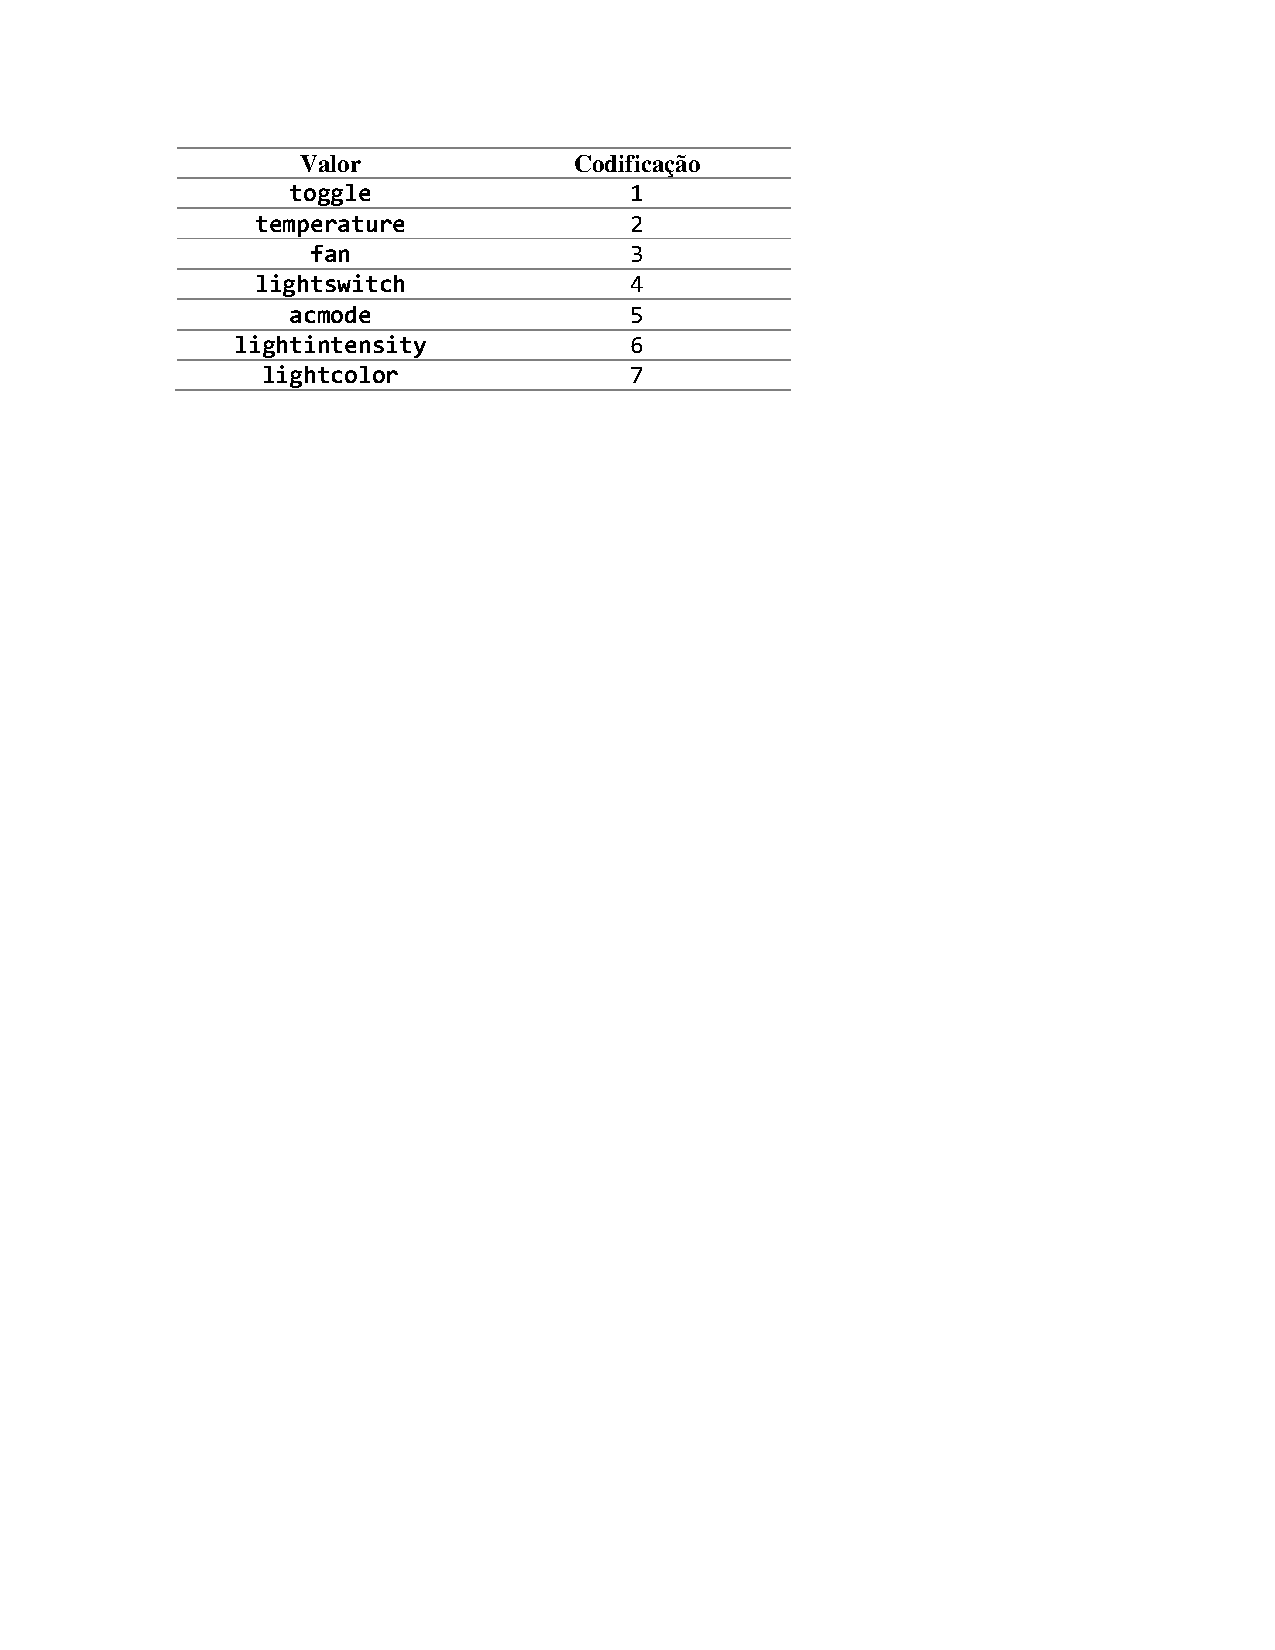
\includegraphics[width=0.7\textwidth]{tabelas/cod_command_category.pdf}
\end{table}

\begin{table}[hp]	
	\centering
	\caption{Codificação de tipos de dados e comandos}\smallskip
	\label{tab:cod_type_category}
	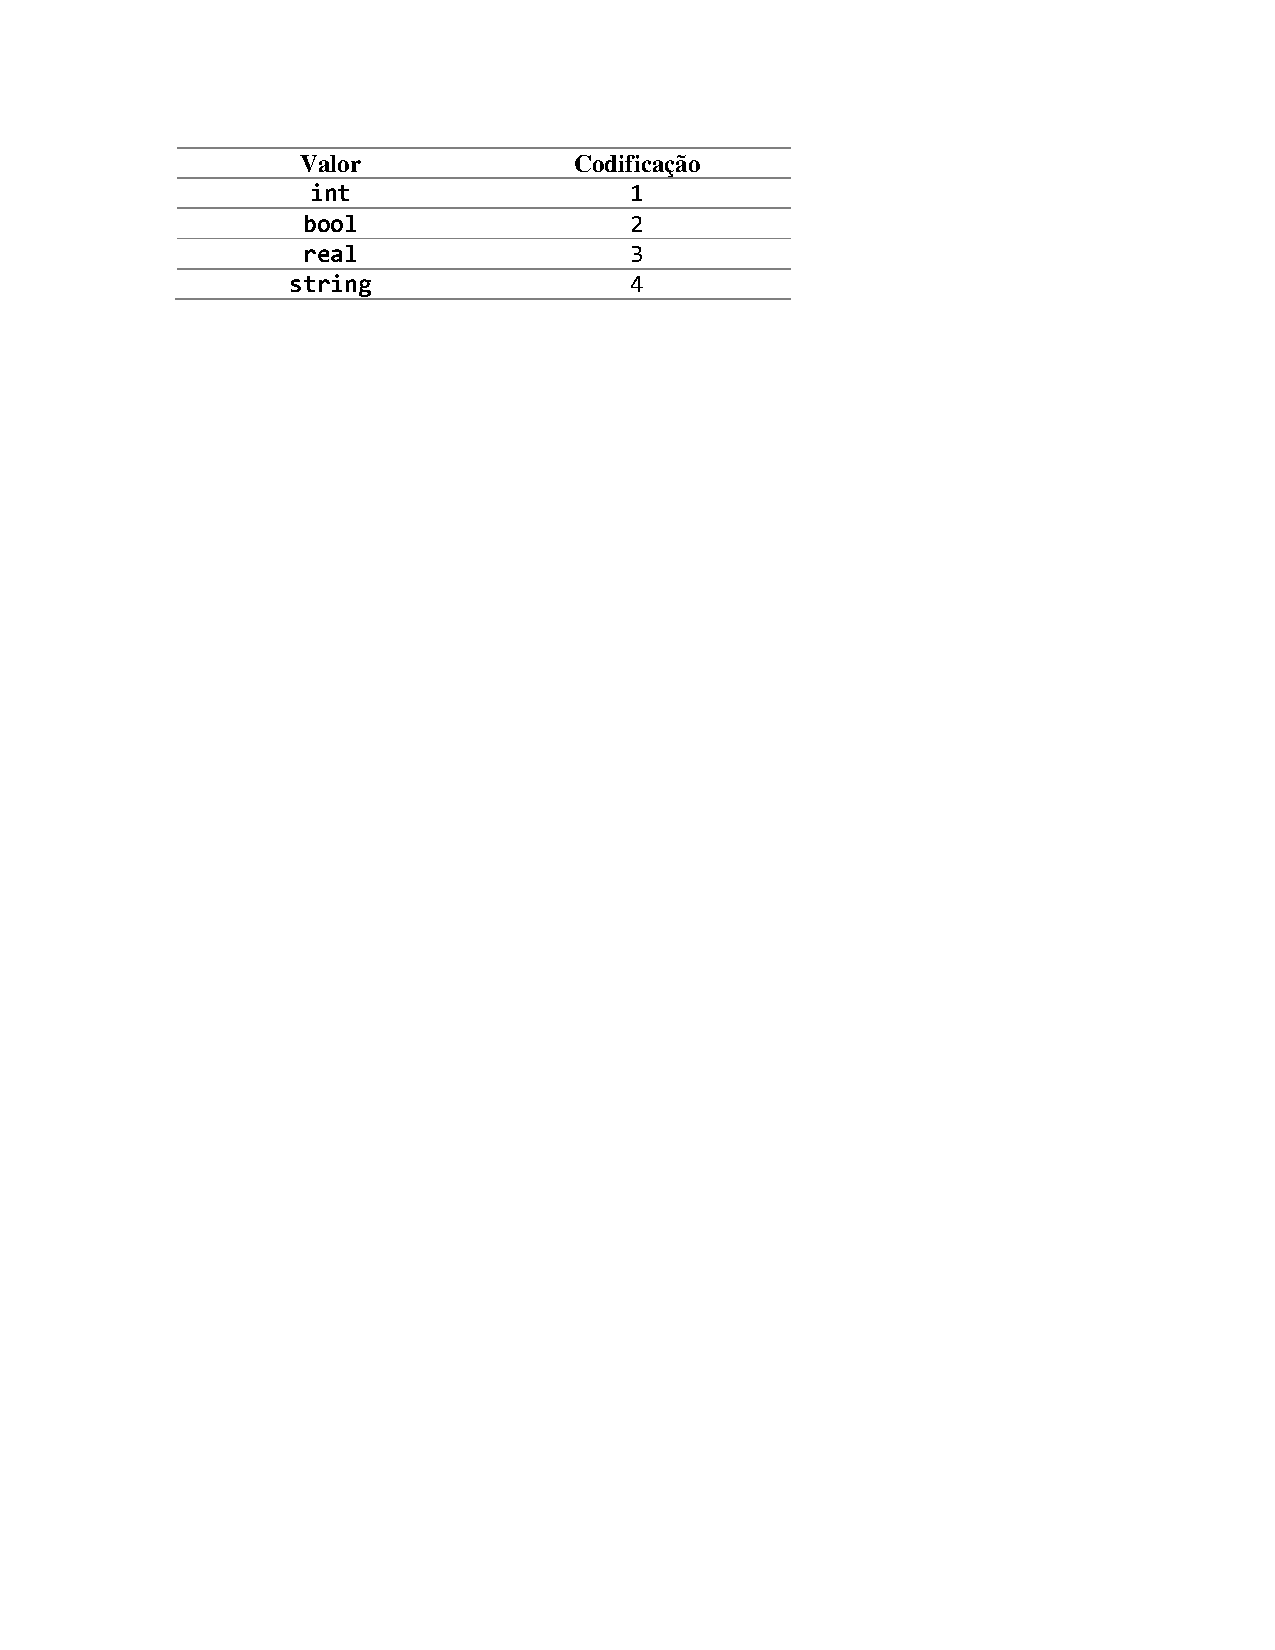
\includegraphics[width=0.7\textwidth]{tabelas/cod_type_category.pdf}
\end{table}

\clearpage
A Figura \ref{fig:tamanho_pacote} mostra os resultados da aplicação das técnicas de compressão de tamanho aos pacotes enviados. No gráfico, são comparados os tamanhos de cada tipo de pacote em três codificações: JSON original (todos os campos são \textit{strings} legíveis), JSON com campos e valores mapeados conforme documentado nesta seção, e JSON mapeado seguido da aplicação da codificação CBOR.

\begin{figure}[h]
	\centering
	\caption{Tamanho resultante do pacote em função da codificação aplicada}
	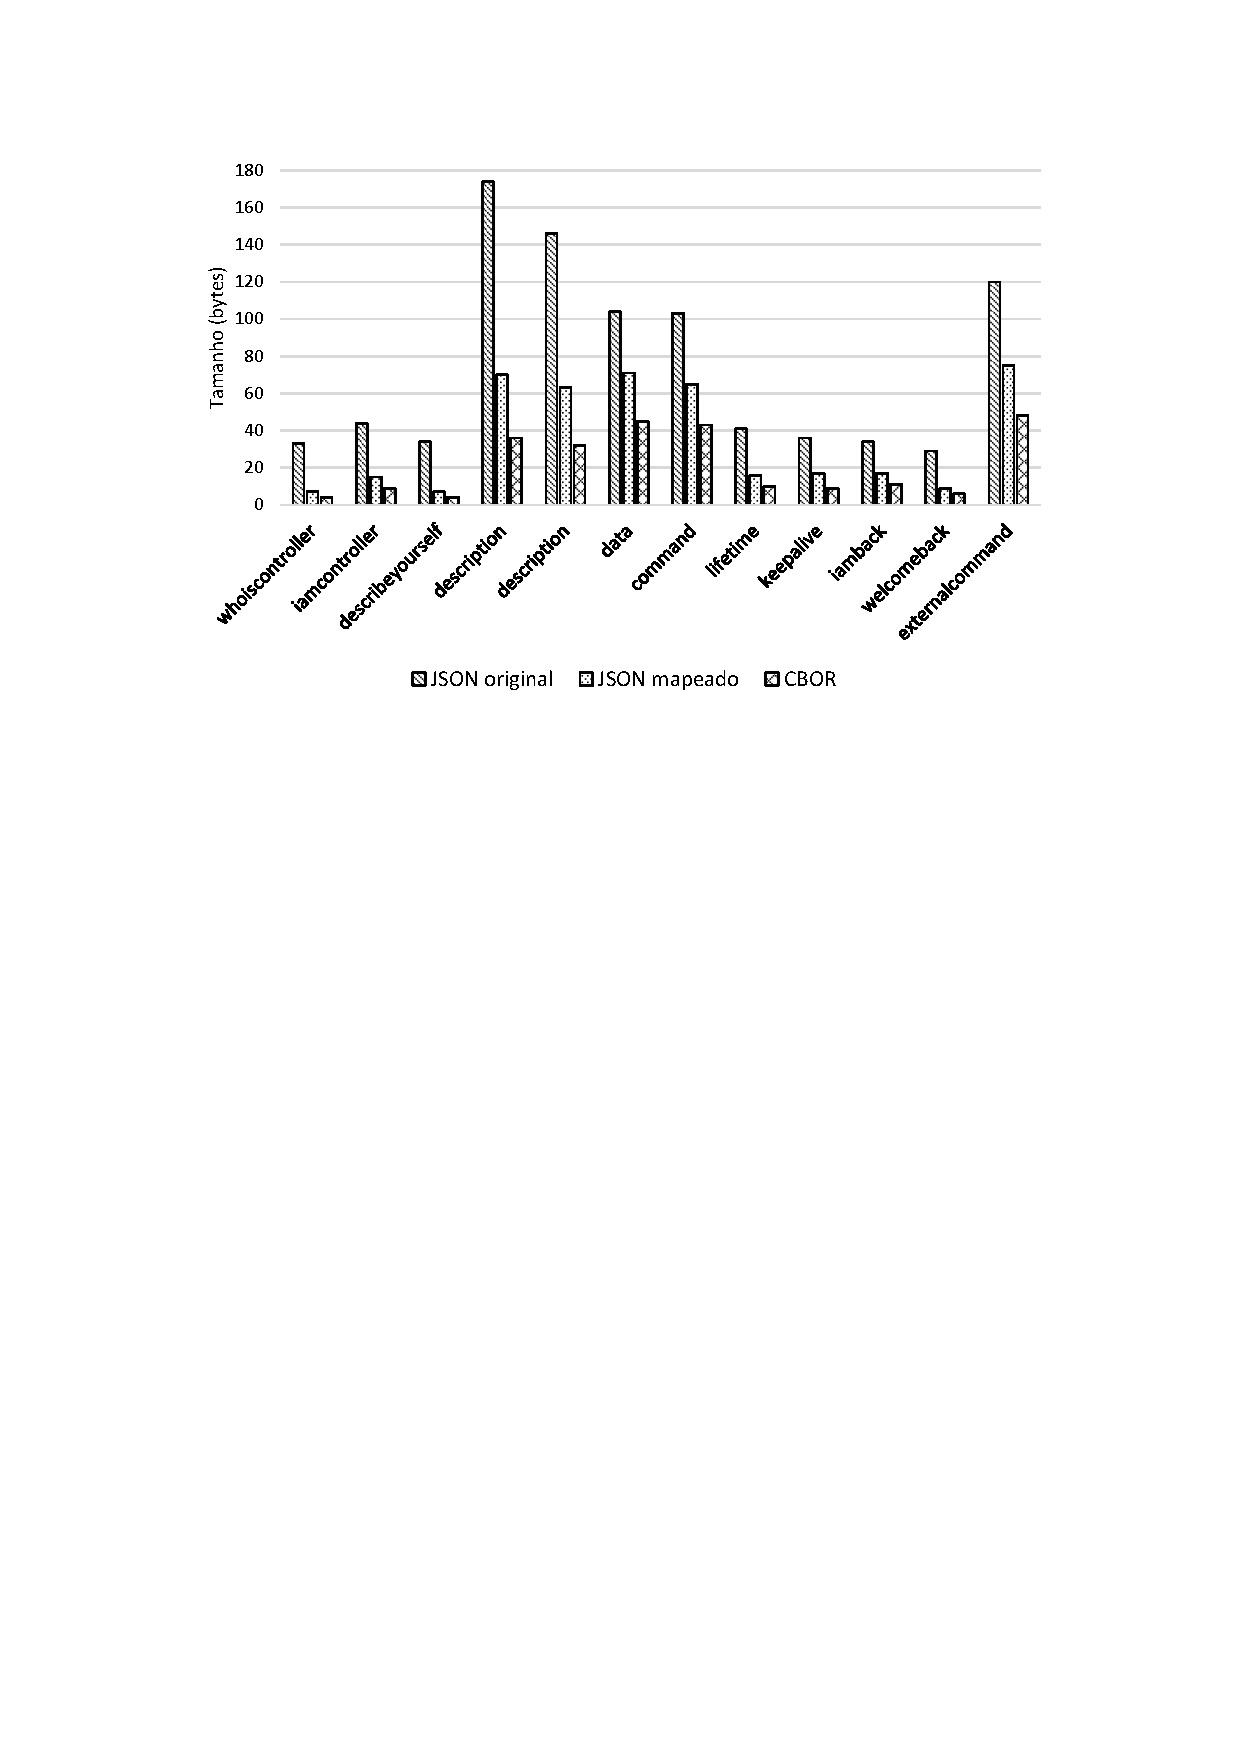
\includegraphics[width=\textwidth]{imagens/tamanho_pacote.pdf}
 	\label{fig:tamanho_pacote}
\end{figure}

Do gráfico, verifica-se que houve redução média de aproximadamente 74\% no tamanho dos pacotes, representando uma redução significativa na quantidade de dados transmitidos na rede. No entanto, em termos práticos, espera-se que pacotes do tipo \texttt{data} e \texttt{command} sejam os mais frequentes em uma rede, visto que os demais ocorrem principalmente durante o \textit{handshake} inicial. A redução de tamanho verificada nestes pacotes foi de 56\% e 58\%, respectivamente, logo espera-se que haja uma redução efetiva no tamanho dos pacotes próxima a esses valores. 

\subsection{Exemplo de Funcionamento}
Para ilustrar o funcionamento do protocolo, considere a rede mostrada na Figura \ref{fig:exemplo_rede}. Nesta rede, existem um sensor (botão), um atuador (interruptor de luz) e um controlador local interligando-os. O botão funciona como um sensor com estado binário: a cada acionamento, seu estado é invertido. De modo similar, o interruptor aceita comandos em formato binário, fechando o contato caso um comando ``1'' seja recebido e abrindo caso ``0'' seja recebido.

\begin{figure}[h]
	\centering
	\caption{Exemplo de aplicação do protocolo \textit{Rainfall}.}
	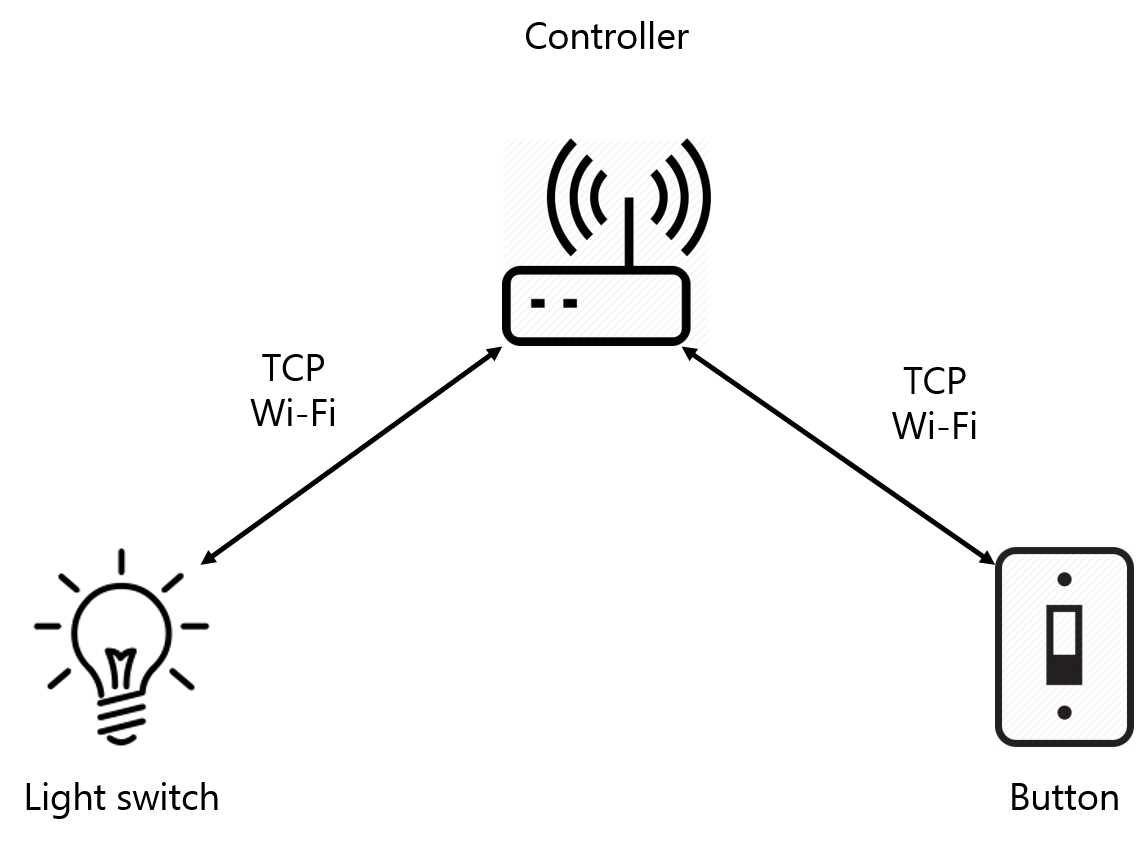
\includegraphics[width=0.7\textwidth]{imagens/exemplo_rede.png}
 	\label{fig:exemplo_rede}
\end{figure}

A Figura \ref{fig:exemplo_handshake} ilustra o processo de \textit{handshake} no exemplo dado. Observe que as mensagens já exploram a possibilidade de enviar múltiplas mensagens em um mesmo pacote, tal como mostrado na Figura \ref{fig:uml_handshake}.

\begin{figure}[hp]
	\centering
	\caption{Processo de \textit{handshake} no exemplo.}
	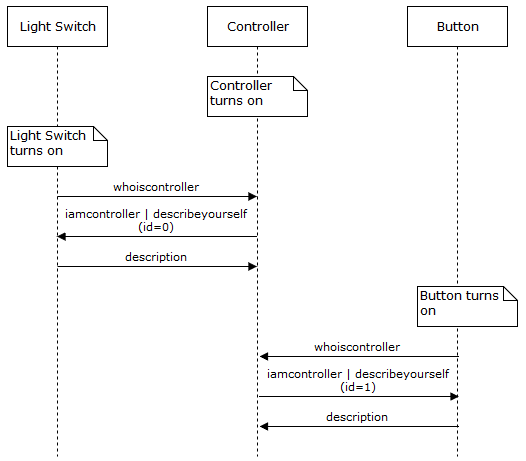
\includegraphics[width=0.9\textwidth]{imagens/exemplo_handshake.png}
 	\label{fig:exemplo_handshake}
\end{figure}

A Figura \ref{fig:exemplo_dados} ilustra o processo de troca de dados e o envio de comandos na rede de exemplo. No caso, o controlador foi configurado com as seguintes regras:
\begin{itemize}
	\item Caso o botão envie um dado ``0'', o comando ``0'' (abrir contato ou apagar a luz) é enviado ao interruptor;
	\item Caso o botão envie um dado ``1'', o comando ``1'' (fechar contato ou acender a luz) é enviado ao interruptor.
\end{itemize}

\begin{figure}[hp]
	\centering
	\caption{Processo de troca de dados e aplicação de regras no exemplo.}
	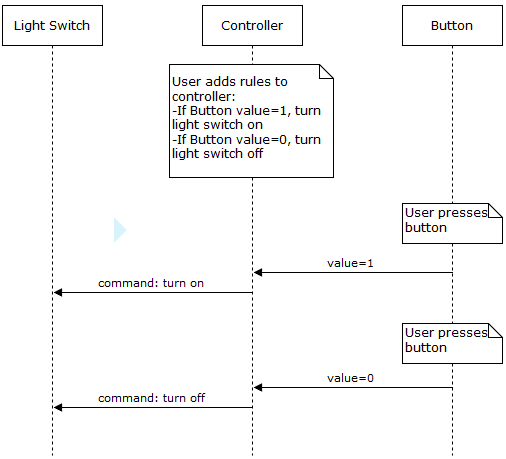
\includegraphics[width=0.9\textwidth]{imagens/exemplo_dados.png}
 	\label{fig:exemplo_dados}
\end{figure}

\clearpage

\section{Implementação de Bibliotecas para o Protocolo de Aplicação} \label{sec:implsens}
Uma vez analisados os protocolos de comunicação existentes e definido o protocolo de aplicação, passa-se para o projeto de uma biblioteca que permita o desenvolvimento de dispositivos em conformidade com ele.

\subsection{Arquitetura}
A biblioteca desenvolvida possuirá uma arquitetura em camadas, conforme ilustra a Figura \ref{fig:libarchitecture}. As camadas apresentadas em cor verde compõem a biblioteca a ser desenvolvida no projeto. A descrição de cada camada está apresentada a seguir.

\begin{figure}[h]
	\centering
	\caption{Arquitetura em camadas da biblioteca}
	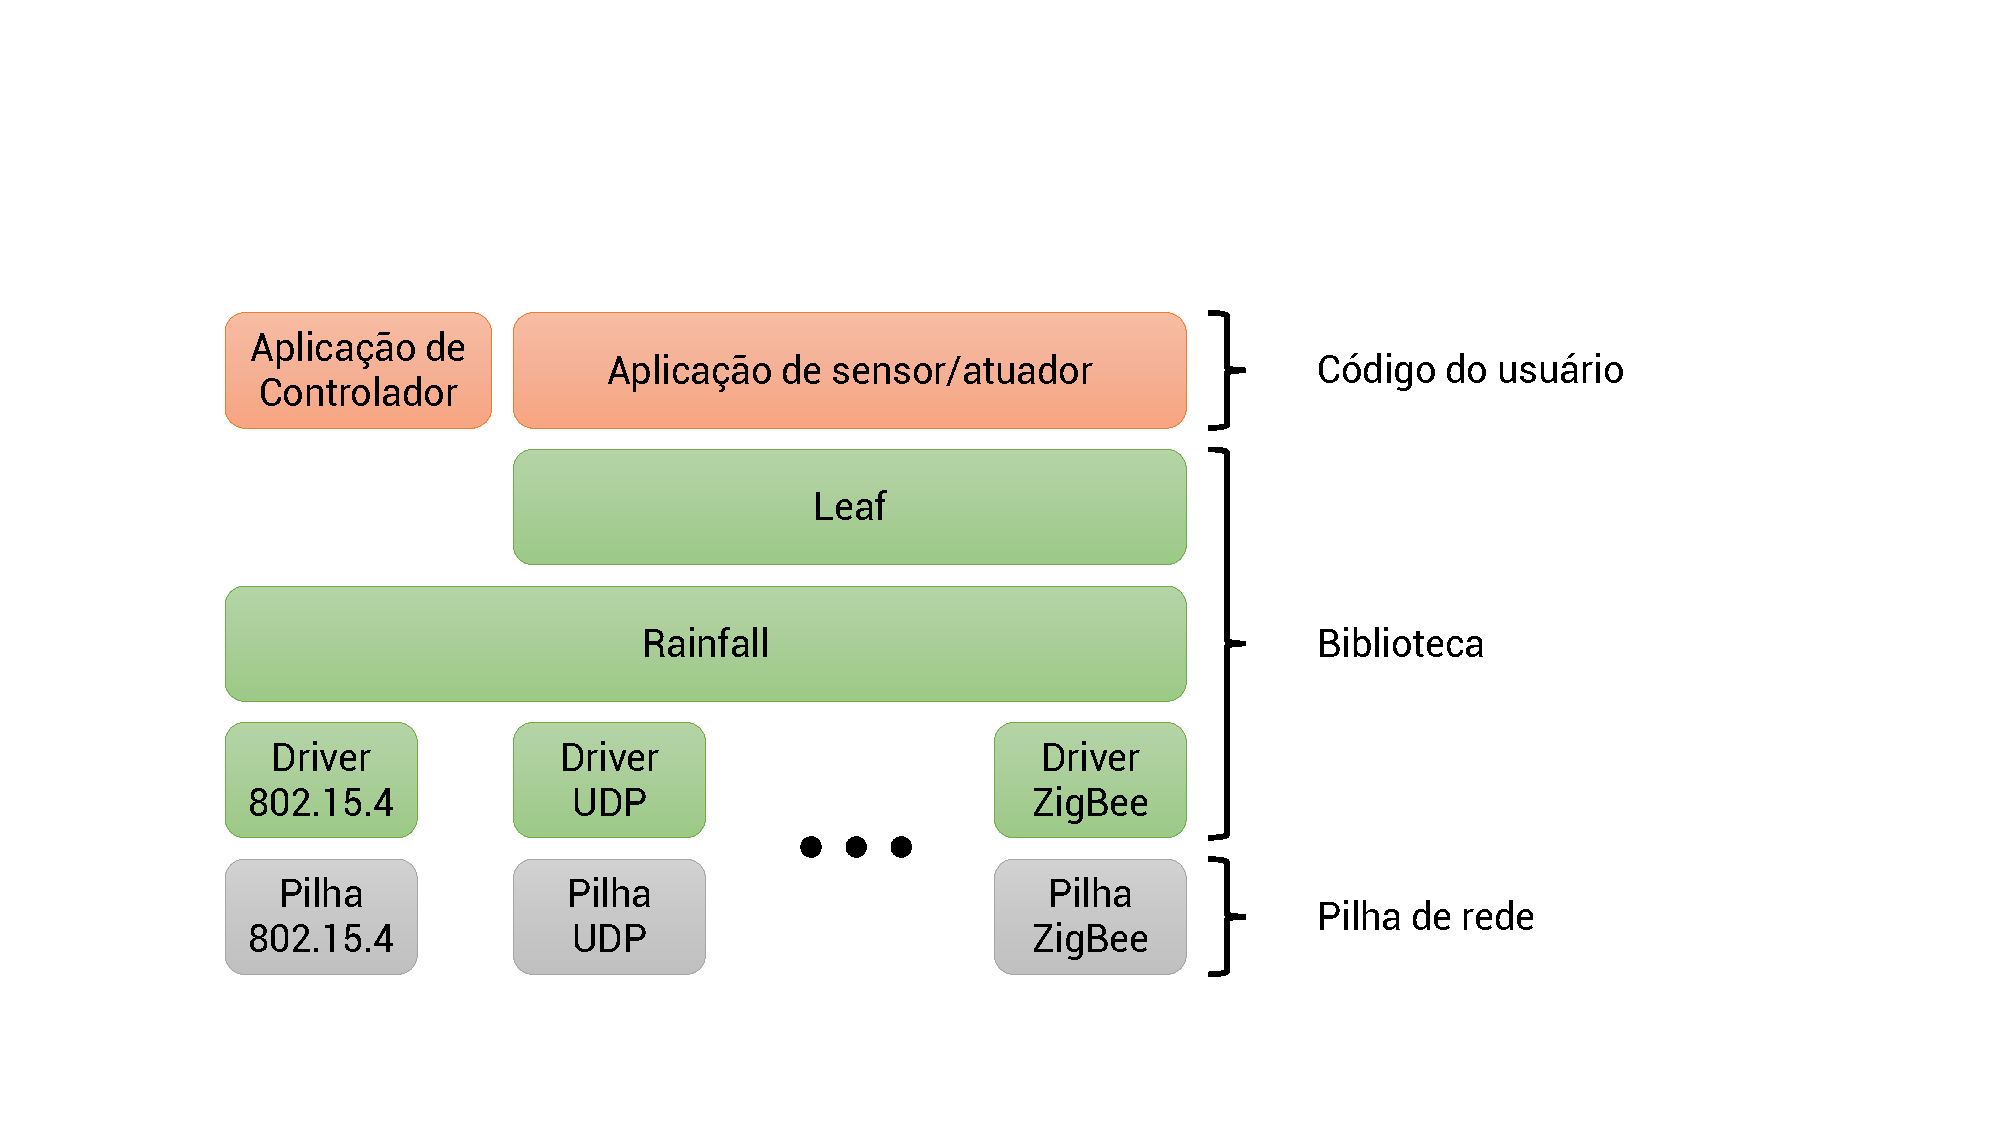
\includegraphics[width=0.8\textwidth]{imagens/libarchitecture.pdf}
 	\label{fig:libarchitecture}
\end{figure}

\paragraph*{Drivers de rede.} A primeira camada da biblioteca consiste em drivers de rede, que proveem uma interface com as diferentes pilhas de rede existentes (cf. item \ref{sec:commprot}). Esta é a única camada da biblioteca que possui dependências com as particularidades de cada protocolo ou dispositivo de rede. Possui a função de prover um acesso uniformizado para funções comuns utilizadas pelas camadas superiores, tais como escutar e enviar pacotes.

\paragraph*{Biblioteca \textit{Rainfall}.} Esta camada tem como objetivo efetuar a transformação de um objeto estruturado segundo as especificações do protocolo \textit{Rainfall} e codificá-lo no formato de envio (mapeando campos e valores para números, e codificando no formato CBOR), e vice-versa. Além disso, ele efetua checagens sintáticas dos pacotes enviados, verificando se somente campos permitidos são utilizados para cada tipo de pacote, conforme as regras apresentadas no item \ref{subsec:sintaxe}. Observe que esta camada atua como um \textit{middleware}, provendo uma interface comum entre a lógica de aplicação e os diversos protocolos de rede.

\paragraph*{Biblioteca \textit{Leaf}.} Esta camada atua sobre as funções fornecidas pela \textit{Rainfall}, fornecendo uma API que abstrai os detalhes do protocolo. Por exemplo, o processo de inicialização mostrado na Figura \ref{fig:uml_handshake} é abstraído através de um método de inicialização disponibilizado nesta biblioteca.

\paragraph*{Aplicações de usuário.} As bibliotecas desenvolvidas permitem o desenvolvimento de \textit{software} de controle de dispositivos em conformidade com as especificações do protocolo \textit{Rainfall}. Dispositivos sensores e atuadores podem ser desenvolvidos facilmente através da biblioteca \textit{Leaf}, ao passo que a lógica de um dispositivo controlador pode ser descrita utilizando-se a biblioteca \textit{Rainfall} diretamente.

\subsection{Implementação e Exemplos}
Uma implementação das bibliotecas para desenvolvimento de dispositivos seguindo o protocolo \textit{Rainfall} foi feita utilizando a linguagem JavaScript, utilizando o ambiente Node.js\footnote{Disponível em \url{https://nodejs.org/}.}. O código-fonte desta implementação, além de exemplos de uso da biblioteca para o desenvolvimento de sensores, atuadores e controladores, estão hospedados no serviço GitHub \footnote{Disponível no endereço \url{https://github.com/HomeSkyLtd/}}.

\section{Limitações e Não-escopos}
O projeto do protocolo de comunicação foi feito com o objetivo de prover um meio de troca de informações entre dispositivos e controladores de uma rede de sensores. Entretanto, dado o contexto de um projeto de conclusão de curso, alguns aspectos não foram enfatizados no presente momento, a despeito de sua importância em aplicações reais. O grupo adotou algumas hipóteses simplificadoras, listadas nas seções a seguir.

\subsection{Conectividade} \label{subsec:limit_conectividade}
As seguintes hipóteses foram feitas no quesito de conectividade dos dispositivos:
\begin{itemize}
	\item Nós se encontram conectados à rede. No projeto do protocolo e na implementação das bibliotecas, não se tratou o processo de conexão dos dispositivos à rede em que o controlador opera. Ou seja, foi considerado que o usuário é capaz de conectar os dispositivos à rede desejada. Existem tecnologias que permitem efetuar conexão de um dispositivo à rede sem necessidade de interface gráfica ou inserção de senhas, tal como o Wi-Fi Protected Setup (WPS), que podem ser utilizados para este fim;
	\item Protocolos de comunicação e/ou transporte subjacentes são confiáveis. No projeto do protocolo, não se tratou o reconhecimento de entrega das mensagens, pois supôs-se que os protocolos de rede ou transporte subjacentes ao de aplicação garantem entrega dos pacotes ao destinatário. Essa é uma estimativa razoável, visto que os protocolos de rede para redes de sensores sem fio assumem que as condições de transmissão são adversas, e incluem mecanismos de retransmissão. No entanto, caco se deseje utilizar um protocolo não confiável, como o UDP, seria possível adicionar um mecanismo de envio de ACKs em nível de aplicação para garantir a entrega.
\end{itemize}

\subsection{Segurança} \label{subsec:limit_seguranca}
As seguintes hipóteses foram feitas no quesito de segurança do sistema:
\begin{itemize}
	\item A infraestrutura de rede é segura. O grupo assumiu que a rede onde os dispositivos atuarão é configurada de forma segura, utilizando algoritmos criptográficos e senhas adequadas. Deste modo, usuários não autorizados ou mal-intencionados não seriam capazes de conectar dispositivos à rede de sensores doméstica. Um modo de tratar o caso em que redes inseguras são utilizadas seria enviar notificações ao usuário a cada nó novo conectado, perguntando se a conexão ao controlador deve ser permitida;
	\item Nós da rede atuam conforme esperado. Supõe-se que nós de rede sejam configurados para operar em conformidade com o protocolo. Por exemplo, um sensor não responderia a mensagens destinadas a outros dispositivos, ou não fingiria ser o controlador. Uma maneira de se assegurar tal comportamento ``honesto'' seria através da efetuação de homologação de dispositivos.
\end{itemize}